\chapter{Convolutional neural networks and deep visual representations}
\label{sec:convolutional_neural_networks}

In Chapter~\ref{sec:deep_feedforward_and_backpropagation}, we established that Multi-Layer Perceptrons equipped with non-linear activation functions are universal function approximators: given sufficient neurons, they can represent any continuous manifold. Yet, in empirical computer vision, deploying dense MLPs directly onto pixel arrays yields an immediate, catastrophic failure. Fully connected networks treat each input feature independently; they possess zero awareness of geometry, spatial adjacency, or physical symmetries.

To construct visual recognition systems that generalize efficiently, machine learning must abandon unconstrained fully connected architectures and embed the physical invariances of the natural visual world directly into the network topology. This breakthrough is realized through \textbf{Convolutional Neural Networks (CNNs)}.

From Yoshua Bengio's Bayesian perspective, a convolutional network is not merely an engineering heuristic: it is a deep neural network endowed with an \textbf{infinitely strong spatial prior}. By enforcing sparse local interactions, parameter sharing across space, and translation equivariance, CNNs slash parameter counts by orders of magnitude, preserve 2D grid topology, and mirror the hierarchical visual processing discovered in the biological mammalian visual cortex by Hubel and Wiesel.

This chapter provides an exhaustive theoretical and mathematical treatment of convolutional architectures: from continuous convolutions and discrete cross-correlations, through receptive field algebra, $1 \times 1$ bottlenecks, and global average pooling, to landmark architectural evolutions (AlexNet, VGG, ResNet) and the complete taxonomy of visual tasks (classification, detection, and semantic segmentation).

\section{The visual challenge and the structural failure of fully connected networks}
\label{sec:failure_of_fc_on_images}

Having derived Fully Connected Networks (FCNs) in Section~\ref{sec:perceptron_to_fcn}, we now confront an empirical crisis: \textit{why does deploying dense fully connected networks on high-dimensional visual sensory data fail completely?}

\subsection{Why MLPs fail on high-dimensional visual data}
\label{sec:why_mlps_fail_images}

\begin{figure}[H]
\centering
\begin{minipage}{0.48\linewidth}
  \centering
  \begin{tikzpicture}[scale=0.88]
    \node[font=\footnotesize\bfseries\color{politoNavy}] at (2.2, 3.4) {(a) Dense Layer (Flattened Vector)};

    % 2D Image Grid
    \draw[fill=gray!10, draw=gray!60, thick] (0, 0.5) rectangle (1.6, 2.1);
    \node[font=\tiny, align=center] at (0.8, 1.3) {$32 \times 32 \times 3$\\Image};

    % Flatten Arrow
    \draw[-{Stealth}, thick, gray!70] (1.7, 1.3) -- (2.3, 1.3) node[midway, above, font=\tiny] {Flatten};

    % 1D Vector (d = 3072)
    \draw[fill=deepblue!20, draw=deepblue, thick] (2.5, -0.4) rectangle (2.9, 3.0);
    \node[font=\tiny, rotate=90] at (2.7, 1.3) {Vector: $3072 \times 1$};

    % Dense Connections
    \foreach \y in {0.0, 0.8, 1.6, 2.4} {
      \draw[gray!40, thin] (2.9, \y) -- (4.2, 2.0);
      \draw[gray!40, thin] (2.9, \y) -- (4.2, 1.2);
      \draw[gray!40, thin] (2.9, \y) -- (4.2, 0.4);
    }

    % Hidden Vector
    \draw[fill=intuitiongreen!20, draw=intuitiongreen, thick] (4.2, 0.0) rectangle (4.6, 2.4);
    \node[font=\tiny, rotate=90] at (4.4, 1.2) {Hidden: $1024 \times 1$};

    \node[font=\scriptsize\color{examred}, align=center] at (2.2, -1.0) {Destroys 2D topology\\$3.15 \times 10^6$ weights};
  \end{tikzpicture}
\end{minipage}\hfill
\begin{minipage}{0.48\linewidth}
  \centering
  \begin{tikzpicture}[scale=0.88]
    \node[font=\footnotesize\bfseries\color{politoNavy}] at (2.2, 3.4) {(b) Convolutional Layer (3D Volume)};

    % 3D Input Volume: 32x32x3
    \draw[fill=deepblue!15, draw=deepblue, thick] (0, 0) -- (1.6, 0) -- (1.6, 1.6) -- (0, 1.6) -- cycle;
    \draw[fill=deepblue!25, draw=deepblue, thick] (1.6, 0) -- (2.1, 0.5) -- (2.1, 2.1) -- (1.6, 1.6) -- cycle;
    \draw[fill=deepblue!10, draw=deepblue, thick] (0, 1.6) -- (0.5, 2.1) -- (2.1, 2.1) -- (1.6, 1.6) -- cycle;
    \node[font=\tiny, align=center] at (0.8, 0.8) {$32 \times 32$\\$\times 3$};

    % Small 3D Receptive Field Filter: 5x5x3
    \draw[fill=examred!30, draw=examred, thick] (0.4, 0.6) rectangle (0.9, 1.1);
    \node[font=\tiny\color{examred}] at (0.65, 0.85) {$F$};

    % Filter arrow
    \draw[-{Stealth}, very thick, examred] (1.1, 0.85) -- (2.8, 0.85);

    % 3D Output Feature Volume
    \draw[fill=intuitiongreen!15, draw=intuitiongreen, thick] (3.0, 0.2) -- (4.2, 0.2) -- (4.2, 1.4) -- (3.0, 1.4) -- cycle;
    \draw[fill=intuitiongreen!25, draw=intuitiongreen, thick] (4.2, 0.2) -- (4.6, 0.6) -- (4.6, 1.8) -- (4.2, 1.4) -- cycle;
    \draw[fill=intuitiongreen!10, draw=intuitiongreen, thick] (3.0, 1.4) -- (3.4, 1.8) -- (4.6, 1.8) -- (4.2, 1.4) -- cycle;
    \node[font=\tiny, align=center] at (3.6, 0.8) {$28 \times 28$\\$\times 6$};

    \node[font=\scriptsize\color{intuitiongreen}, align=center] at (2.2, -1.0) {Preserves 3D spatial grid\\Reuses shared weights};
  \end{tikzpicture}
\end{minipage}
\caption{The structural contrast between dense and convolutional representations. (a) A dense fully connected layer flattens an image into an unrolled 1D vector, destroying all 2D spatial adjacency and requiring an independent weight for every pixel-neuron pair. (b) A convolutional layer preserves the native 3D tensor volume, sliding localized spatial filters across coordinates with shared parameters.}
\label{fig:dense_vs_conv_geometry}
\end{figure}

As illustrated in Figure~\ref{fig:dense_vs_conv_geometry}, standard fully connected networks suffer from three crippling structural flaws when applied to visual data:

\paragraph{1. The Vectorization Requirement and Destruction of 2D Spatial Topology.}
To ingest visual sensory data into a Multi-Layer Perceptron, one must reconcile a fundamental dimensional mismatch. An artificial neuron computes an affine inner product followed by an element-wise activation:
\begin{equation}
z = \mathbf{w}^\top \mathbf{x} + b = \sum_{k=1}^d w_k x_k + b.
\end{equation}
Because the canonical Euclidean inner product and standard matrix-vector multiplication $\mathbf{W}\mathbf{x}$ are defined exclusively over one-dimensional coordinate vectors $\mathbf{x} \in \R^d$, a dense layer \textbf{cannot natively ingest multidimensional array grids}. 

Consequently, any multi-channel visual input tensor $\mathbf{X} \in \R^{H \times W \times C}$ must undergo mandatory \textbf{vectorization (flattening)} into an unrolled 1D column vector:
\begin{equation}
\mathbf{x} = \operatorname{vec}(\mathbf{X}) \in \R^{d}, \quad \text{where } d = H \cdot W \cdot C,
\label{eq:flattening_transformation}
\end{equation}
under which each spatial coordinate $(i, j)$ in channel $c$ is mapped to a serialized linear index $k(i, j, c) = c \cdot (HW) + i \cdot W + j$.

This flattening operation fundamentally shatters the geometrical structure of the image:
\begin{itemize}[leftmargin=*]
  \item \textbf{Metric Space Disruption}: In the native continuous 2D image plane, geometry is governed by the standard Euclidean distance metric between pixel coordinates:
  \begin{equation}
  d_{\text{spatial}}(\mathbf{p}_1, \mathbf{p}_2) = \|\mathbf{p}_1 - \mathbf{p}_2\|_2 = \sqrt{(i_1 - i_2)^2 + (j_1 - j_2)^2}.
  \end{equation}
  Pixels that are immediate vertical neighbors, such as $(i, j)$ and $(i+1, j)$, have a spatial distance of $1$. However, in the flattened vector $\mathbf{x}$, their serialized indices are separated by an entire row of $W$ elements: $|k_1 - k_2| = W$. Conversely, pixels at the end of one row $(i, W)$ and the start of the next row $(i+1, 1)$ appear adjacent in 1D index space ($|k_1 - k_2| = 1$), despite residing on opposite physical edges of the image!
  \item \textbf{Loss of Locality and Spatial Adjacency}: Natural visual semantics (edges, textures, object contours) emerge entirely from \textbf{local spatial coherence}: adjacent pixels share physical illumination, surface reflectance, and material properties. By discarding the 2D grid, an MLP discards the concept of a neighborhood $\mathcal{N}(i, j)$, treating a pixel's relationship with its immediate neighbor identically to its relationship with a distant pixel hundreds of scanlines away.
  \item \textbf{The Permutation Invariance Flaw}: Because a dense weight matrix $\mathbf{W} \in \R^{M \times d}$ assigns an unconstrained independent parameter $W_{m, k}$ to every coordinate $k$, an MLP possesses \textbf{zero spatial inductive bias}. To demonstrate this formally, let $\mathbf{P}_\pi \in \{0, 1\}^{d \times d}$ be an arbitrary fixed permutation matrix that randomly shuffles the $d$ pixel indices, transforming every image into humanly unrecognizable white noise static. If we simultaneously permute the columns of the weight matrix by $\mathbf{W}' = \mathbf{W}\mathbf{P}_\pi^\top$, then for any scrambled input $\mathbf{x}' = \mathbf{P}_\pi \mathbf{x}$:
  \begin{equation}
  \mathbf{W}' \mathbf{x}' = (\mathbf{W}\mathbf{P}_\pi^\top)(\mathbf{P}_\pi \mathbf{x}) = \mathbf{W}(\mathbf{P}_\pi^\top \mathbf{P}_\pi)\mathbf{x} = \mathbf{W}\mathbf{x}.
  \end{equation}
  The MLP produces the \textit{exact same forward pre-activations, the exact same backpropagated gradients, and the exact same loss trajectory} on scrambled white noise as it does on structured natural images! An MLP cannot tell whether its input was a photographic scene or a scrambled column of tabular database numbers.
\end{itemize}

\paragraph{2. Zero Weight Sharing and Total Lack of Translation Equivariance.}
In an unconstrained dense layer, every hidden neuron $m$ connects to every input coordinate $k = (i, j, c)$ via a unique, dedicated weight parameter $W_{m, (i, j, c)}$:
\begin{equation}
z_m = \sum_{c=1}^C \sum_{i=1}^H \sum_{j=1}^W W_{m, (i, j, c)} X_{i, j, c} + b_m.
\label{eq:dense_coordinate_binding}
\end{equation}
This formulation has two catastrophic consequences:
\begin{itemize}[leftmargin=*]
  \item \textbf{Coordinate-Specific Parameter Binding (Zero Weight Sharing)}: In Equation~\eqref{eq:dense_coordinate_binding}, the weight $W_{m, (i, j, c)}$ is bound to the absolute spatial coordinate $(i, j)$ on the canvas. There is \textbf{zero parameter sharing}: the weight that examines coordinate $(10, 10)$ shares no algebraic relationship with the weight examining coordinate $(150, 150)$. To share parameters across spatial locations, the matrix $\mathbf{W}$ would have to be constrained to have a doubly block-circulant (or Toeplitz) structure---which is precisely the mathematical definition of a discrete convolution! Unconstrained MLPs lack this structure entirely.
  \item \textbf{Breakdown of Translation Equivariance}: Physical objects satisfy \textbf{translational symmetry}: a cat, a pedestrian, or a traffic sign retains identical identity, scale, and visual features regardless of whether it appears in the upper-left corner, the center, or the lower-right corner of the visual field. Mathematically, a representation mapping $f: \mathcal{X} \to \mathcal{H}$ is \textbf{translation-equivariant} with respect to spatial shift $T_{\mathbf{v}}$ if:
  \begin{equation}
  f(T_{\mathbf{v}}(\mathbf{X})) = T_{\mathbf{v}}(f(\mathbf{X})), \quad \forall \mathbf{v} \in \mathbb{Z}^2.
  \end{equation}
  In an MLP, because weights are rigidly tied to absolute pixel coordinates, $f(T_{\mathbf{v}}(\mathbf{x})) \ne T_{\mathbf{v}}(f(\mathbf{x}))$. If a hidden neuron learns a set of weights that successfully detects an eye at coordinates $(10, 10)$, and in a new test image the subject is shifted so the eye appears at $(150, 150)$, the neuron at $(10, 10)$ fails to activate, and the neuron at $(150, 150)$ has never seen an eye during training! The network possesses zero ability to transfer learned patterns across spatial coordinates.
  \item \textbf{Exponential Sample Complexity}: Because an MLP cannot share parameters across space, it cannot generalize across translations. To learn that an object can appear anywhere on the canvas, the MLP must observe that object at \textbf{every possible spatial coordinate $(i, j)$ during training}. This multiplies the required training dataset size by a factor proportional to the spatial resolution $H \times W$, making sample-efficient visual learning impossible.
\end{itemize}

\paragraph{3. Catastrophic Parameter Explosion and Overfitting.}
The combination of all-to-all dense connectivity and zero parameter sharing inevitably triggers a catastrophic parameter explosion:
\begin{equation}
N_{\text{weights}} = d_{\text{in}} \times d_{\text{out}} = (H \cdot W \cdot C) \times M,
\end{equation}
where $M$ is the number of neurons in the first hidden layer.
\begin{itemize}[noitemsep]
  \item \textbf{Small Resolution (CIFAR-10)}: For a tiny $32 \times 32 \times 3$ thumbnail ($d = 3,072$), connecting to a hidden layer of $M = 1,024$ neurons requires $3,072 \times 1,024 \approx 3.15 \times 10^6$ parameters.
  \item \textbf{Medium Resolution ($256 \times 256 \times 3$)}: Here, $d = 196,608$. Connecting to a modest hidden layer of $M = 2,048$ neurons requires:
    \begin{equation}
    196,608 \times 2,048 = 402,653,184 \text{ parameters (over } 402 \text{ million weights!)}
    \end{equation}
    for the \textbf{first layer alone}! Storing this single weight matrix in 32-bit floating point precision consumes over $1.61\text{ GB}$ of VRAM.
  \item \textbf{High Resolution (Full HD $1080 \times 1920 \times 3$)}: $d \approx 6.22 \times 10^6$. A single hidden layer of $2,048$ neurons would require over $1.27 \times 10^{10}$ parameters (12.7 billion weights, $\sim 50\text{ GB}$ of memory).
\end{itemize}
By Vapnik-Chervonenkis (VC) generalization theory (Chapter~\ref{sec:pac_learning_theory}), the sample complexity required to prevent overfitting scales linearly with the number of free parameters ($N \propto \mathcal{O}(|\boldsymbol{\theta}|)$). Training an unconstrained model with hundreds of millions of parameters on typical dataset sizes ($N \sim 10^4$--$10^6$) guarantees catastrophic overfitting and failure to generalize.

\subsection{Natural image statistics: Why do all images share universal patterns?}
\label{sec:natural_image_statistics}

Why are dense networks structurally mismatched to images, and why can we design a far more compact, universal visual architecture? As Prof.~Tatiana Tommasi emphasized during lectures, the answer lies in the fundamental statistical physics of natural scenes.

\paragraph{1. Natural Images vs. White Noise.}
An arbitrary $256 \times 256$ RGB image can take $(256)^{256 \times 256 \times 3} \approx 10^{473,000}$ possible configurations. However, the set of \textbf{natural images} occupies an infinitesimal sub-manifold within this immense space. If pixels were drawn independently from a Gaussian white noise distribution, images would resemble uniform television static, containing zero discernible structures.

Natural images are profoundly non-random because they are optical projections of a \textbf{physical 3D universe}:
\begin{itemize}[noitemsep]
  \item Solid physical objects consist of continuous matter with uniform surface reflectance.
  \item Optical illumination casts smooth gradients across surfaces.
  \item Object occlusions and material boundaries produce sharp, localized step discontinuities.
\end{itemize}

\paragraph{2. Universal Statistical Symmetries of Natural Scenes.}
Empirical investigations into natural image statistics (Ruderman, Simoncelli, Olshausen \& Field) reveal that virtually all natural images share identical mathematical regularities:
\begin{enumerate}
  \item \textbf{High Local Autocorrelation}: The correlation between two pixels $\mathbf{I}(\mathbf{x})$ and $\mathbf{I}(\mathbf{x} + \Delta \mathbf{x})$ approaches $1$ as $\|\Delta \mathbf{x}\|_2 \to 0$. Adjacent pixels almost always possess identical color and luminance; significant differences occur only at boundaries.
  \item \textbf{Scale Invariance and the $1/f^2$ Power Spectrum}: The power spectral density $S(f)$ of natural scenes universally follows a power law:
    \begin{equation}
    S(f) \propto \frac{1}{f^{2 - \eta}}, \quad \text{with } \eta \approx 0.2.
    \label{eq:power_spectrum_law}
    \end{equation}
    This scale-invariant property implies that natural images exhibit identical statistical structure at all spatial scales: low spatial frequencies (broad smooth areas) dominate the energy budget, while high spatial frequencies (edges and fine textures) represent a sparse, highly informative fraction.
  \item \textbf{Universality of Edge Primitives}: Across entirely unrelated domains—whether analyzing portraits, satellite topography, medical histology, or urban streetscapes—the visual world is universally built from the same primitive visual tokens: \textbf{oriented edges, localized step transitions, and corner junctions}.
\end{enumerate}

Because all natural images share these identical low-level statistical regularities, an optimal visual machine learning model should not learn arbitrary, unconstrained dense weights. Instead, it must embody inductive biases that exploit locality, stationarity, and hierarchical compositionality!

\begin{figure}[H]
\centering
\begin{tikzpicture}[scale=0.95]
  % Stage 1: Pixels
  \node[rectangle, draw=gray!80, fill=gray!10, thick, inner sep=6pt, font=\footnotesize, align=center] (s1) at (0, 0) {
    \textbf{Level 1: Raw Pixels}\\
    Coordinate grid $\mathbf{I}(i, j) \in [0, 255]^3$
  };

  % Stage 2: Edges & Contours
  \node[rectangle, draw=deepblue, fill=deepblue!15, thick, inner sep=6pt, font=\footnotesize, align=center] (s2) at (3.5, 0) {
    \textbf{Level 2: Low-Level Primitives}\\
    Oriented edges, bars, Gabor wavelets
  };

  % Stage 3: Motifs & Textures
  \node[rectangle, draw=intuitiongreen, fill=intuitiongreen!15, thick, inner sep=6pt, font=\footnotesize, align=center] (s3) at (7.2, 0) {
    \textbf{Level 3: Mid-Level Motifs}\\
    Corners, junctions, textures, shapes
  };

  % Stage 4: Parts & Objects
  \node[rectangle, draw=politoNavy, fill=politoNavy!20, thick, inner sep=6pt, font=\footnotesize, align=center] (s4) at (11.0, 0) {
    \textbf{Level 4: High-Level Semantics}\\
    Object parts (eyes, wheels) $\to$ Full objects
  };

  % Directed Arrows between stages
  \draw[-{Stealth}, very thick, politoNavy] (s1) -- (s2);
  \draw[-{Stealth}, very thick, politoNavy] (s2) -- (s3);
  \draw[-{Stealth}, very thick, politoNavy] (s3) -- (s4);

  % Receptive Field expansion annotation below
  \draw[thick, deepdiveTeal, {Stealth}-{Stealth}] (0, -0.9) -- (11.0, -0.9);
  \node[font=\scriptsize\bfseries\color{deepdiveTeal}, below=2pt] at (5.5, -0.9) {Increasing Receptive Field \& Semantic Abstraction $\longrightarrow$};
\end{tikzpicture}
\caption{The hierarchical compositionality of visual representations. Natural images are formed compositionally: local pixels combine into oriented edges, edges aggregate into textures and geometric motifs, which assemble into object parts, and ultimately into semantic categories. Convolutional networks emulate this visual hierarchy across cascading layers.}
\label{fig:visual_feature_hierarchy}
\end{figure}

As depicted in Figure~\ref{fig:visual_feature_hierarchy}, neurophysiologists David Hubel and Torsten Wiesel~\cite{hubel1959receptive,hubel1962receptive} discovered in 1959 that the mammalian visual cortex (area V1) is organized precisely according to this compositional principle: \textbf{Simple Cells} respond to localized oriented bars within small receptive fields, while \textbf{Complex Cells} pool over simple cells to achieve local translation tolerance. 
This biological architecture inspired Kunihiko Fukushima's \textbf{Neocognitron} (1980)~\cite{fukushima1980neocognitron} and Yann LeCun's \textbf{LeNet} (1989)~\cite{lecun1989backpropagation}, establishing the mathematical paradigm of \textbf{Convolutional Neural Networks}.

---

\section{Convolution mechanics, algebra, and geometry}
\label{sec:cnn_mechanics_and_geometry}

Having demonstrated the structural failure of dense MLPs and the statistical regularities of natural images, we now introduce the mathematical framework engineered to operationalize these visual priors: \textbf{Convolutional Neural Networks (CNNs)}.

By replacing unconstrained matrix multiplications with discrete cross-correlations, CNNs enforce three foundational physical priors directly into the network architecture:
\begin{enumerate}
  \item \textbf{Sparse Interactions (Locality)}: Rather than connecting each hidden unit to all $H \times W$ pixels, a convolutional filter interacts only with a small, localized spatial patch of size $F \times F$ (typically $3 \times 3$ or $5 \times 5$).
  \item \textbf{Parameter Sharing (Tied Weights)}: Rather than learning separate parameters for every spatial location, the identical filter kernel is reused across every receptive field in the visual grid.
  \item \textbf{Translation Equivariance}: Because the filter slides uniformly across space, translating the input image translates the output representation identically:
    \begin{equation}
    f\left( \mathcal{T}_{(\Delta x, \Delta y)}[\mathbf{X}] \right) = \mathcal{T}_{(\Delta x, \Delta y)}[f(\mathbf{X})].
    \label{eq:equivariance_def}
    \end{equation}
\end{enumerate}

\subsection{The continuous convolution and discrete 2D cross-correlation}
\label{sec:convolution_mathematical_definition}

To establish the theoretical foundations of convolutional neural networks, we must first examine the convolution operation from a rigorous mathematical and physical perspective, tracing its formulation from functional analysis to modern tensor computation~\cite{goodfellow2016deep,bishop2024deep}.

\paragraph{Continuous 1D Convolution and the Spaceship Laser Tracking Analogy.}
In functional analysis, the \textbf{continuous convolution} of two real-valued integrable functions $x, w: \R \to \R$ is defined by the integral:
\begin{equation}
s(t) = (x * w)(t) \triangleq \int_{-\infty}^{\infty} x(\tau) w(t - \tau) \, d\tau.
\label{eq:continuous_convolution}
\end{equation}
In the deep learning terminology established by Goodfellow, Bengio, and Courville~\cite{goodfellow2016deep}, the first function $x(t)$ is referred to as the \textbf{input}, the second function $w(t)$ is known as the \textbf{kernel} (or weighting function), and the resulting output $s(t)$ is referred to as the \textbf{feature map}.

To intuitively grasp why Equation~\eqref{eq:continuous_convolution} possesses this precise functional form, consider Bengio's canonical physical analogy~\cite{goodfellow2016deep}: suppose we are tracking the 1D position of a spaceship across space using an onboard laser rangefinder. At any continuous time $t$, the laser sensor outputs a scalar position measurement $x(t)$. Because laser sensor electronics are inherently subject to high-frequency stochastic noise, any instantaneous measurement $x(t)$ is noisy. To obtain an accurate, stabilized trajectory estimate $s(t)$, we compute a running weighted average of recent sensor readings. 

Naturally, sensor measurements taken recently are far more informative about the spaceship's current location than measurements recorded long ago. Thus, we define a weighting kernel $w(a)$, where $a$ denotes the \textbf{age of the measurement} ($a \ge 0$), designed such that $w(a)$ is large when $a \to 0$ and decays rapidly toward zero as $a \to \infty$. If the current time is $t$ and a past measurement was acquired at timestamp $\tau \le t$, the elapsed age of that specific measurement is precisely:
\begin{equation}
a = t - \tau.
\end{equation}
Weighting each historical observation $x(\tau)$ by the credibility of its age $w(t - \tau)$ and continuously integrating over all history yields the smoothed spaceship position:
\begin{equation}
s(t) = \int_{-\infty}^{\infty} x(\tau) w(t - \tau) \, d\tau = (x * w)(t).
\end{equation}

\paragraph{The Four Mechanical Operations of Convolution.}
Mechanically, evaluating the continuous convolution integral $(f * g)(t)$ at an arbitrary evaluation timestamp $t$ requires four sequential mathematical operations:
\begin{enumerate}[leftmargin=*]
  \item \textbf{Reflection (Time Reversal / Kernel Flip)}: We reflect the kernel function across the vertical axis:
    \begin{equation}
    g(\tau) \mapsto g(-\tau).
    \end{equation}
    This reflection is mathematically fundamental: it ensures that older historical events (smaller $\tau$) are multiplied by weights corresponding to larger elapsed ages ($t - \tau$).
  \item \textbf{Translation (Temporal Displacement)}: We shift the reflected kernel along the time axis by offset $t$:
    \begin{equation}
    g(-\tau) \mapsto g(-(\tau - t)) = g(t - \tau).
    \end{equation}
  \item \textbf{Pointwise Multiplication}: We evaluate the instantaneous pointwise product of the original signal $f(\tau)$ and the shifted, reflected kernel $g(t - \tau)$ across all $\tau$:
    \begin{equation}
    h_t(\tau) = f(\tau) \cdot g(t - \tau).
    \end{equation}
  \item \textbf{Integration (Area Accumulation)}: We compute the total definite integral (the net area under the product curve $h_t(\tau)$) over the entire real line:
    \begin{equation}
    (f * g)(t) = \int_{-\infty}^{\infty} h_t(\tau) \, d\tau.
    \end{equation}
\end{enumerate}

\begin{figure}[H]
\centering
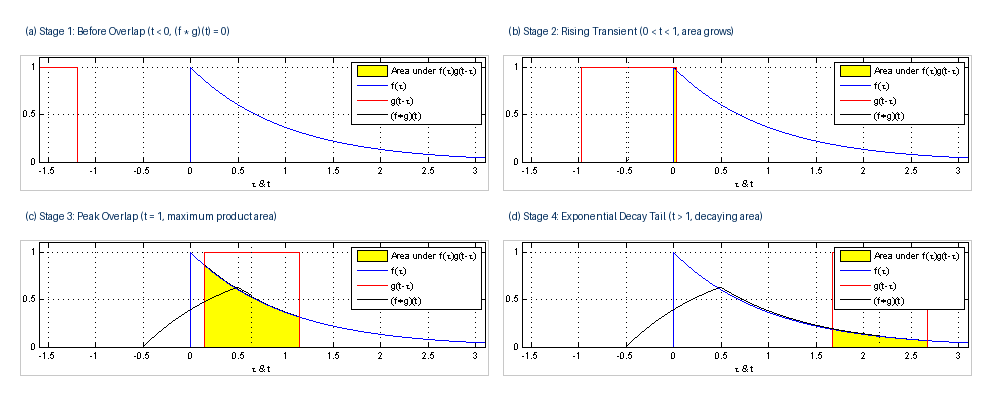
\includegraphics[width=\linewidth]{figures/wikipedia_convolution_animation.png}
\caption{Continuous 1D convolution of a spiky signal $f(\tau)$ with a symmetric box kernel $g(\tau)$ over displacement $t$, illustrating the four mechanical phases: (a) Stage 1: Before Overlap ($t < 0$), where the disjoint supports yield $(f * g)(t) = 0$; (b) Stage 2: Rising Transient ($0 \le t \le 1$), where the leading edge sweeps across the spiky signal and the overlapping area grows; (c) Stage 3: Peak Overlap ($t = 1$), where maximal mass of the spiky signal is contained inside the kernel window, maximizing the integral; (d) Stage 4: Exponential Decay Tail ($t > 1$), where the lagging edge leaves the spiky peak and the integral decays asymptotically. Source: Wikimedia Commons (\href{https://commons.wikimedia.org/wiki/File:Convolution_of_spiky_function_with_box2.gif}{Convolution of spiky function with box2.gif}).}
\label{fig:wikipedia_convolution_animation}
\end{figure}

\paragraph{Continuous 2D Convolution and Algebraic Properties.}
Extending this formulation to continuous 2D functional spaces (such as continuous optical wavefields $\R^2 \to \R$), continuous 2D convolution integrates over both spatial dimensions:
\begin{equation}
S(x, y) = (I * K)(x, y) \triangleq \int_{-\infty}^{\infty} \int_{-\infty}^{\infty} I(\tau_x, \tau_y) K(x - \tau_x, \, y - \tau_y) \, d\tau_x \, d\tau_y.
\label{eq:continuous_2d_convolution}
\end{equation}
Continuous convolution satisfies three foundational algebraic properties:
\begin{itemize}[leftmargin=*]
  \item \textbf{Commutativity}: $f * g = g * f$. By performing the change of variables $u = t - \tau$ (hence $du = -d\tau$):
    \begin{equation}
    (f * g)(t) = \int_{-\infty}^{\infty} f(\tau) g(t - \tau) \, d\tau = \int_{\infty}^{-\infty} f(t - u) g(u) (-du) = \int_{-\infty}^{\infty} g(u) f(t - u) \, du = (g * f)(t).
    \label{eq:convolution_commutativity_proof}
    \end{equation}
  \item \textbf{Associativity}: $f * (g * h) = (f * g) * h$. Cascading linear time-invariant filters can be collapsed into a single equivalent filter $k = g * h$.
  \item \textbf{Distributivity}: $f * (g + h) = (f * g) + (f * h)$.
\end{itemize}

\paragraph{Discrete 2D Cross-Correlation in Deep Learning.}
In computer vision, digital images are discrete 2D matrices of sampled pixel intensities $\mathbf{I} \in \R^{H \times W}$, and filters are discrete 2D tensors $\mathbf{K} \in \R^{F \times F}$. Replacing the continuous integrals with discrete summations, the formal mathematical discrete convolution is:
\begin{equation}
S(i, j) = (\mathbf{I} * \mathbf{K})(i, j) \triangleq \sum_{m=-\infty}^{\infty} \sum_{n=-\infty}^{\infty} \mathbf{I}(m, n) \, \mathbf{K}(i - m, \, j - n).
\label{eq:discrete_convolution_true}
\end{equation}
Because the sum is commutative, Equation~\eqref{eq:discrete_convolution_true} can be equivalently evaluated by flipping the kernel indices:
\begin{equation}
S(i, j) = (\mathbf{K} * \mathbf{I})(i, j) = \sum_{m} \sum_{n} \mathbf{I}(i - m, \, j - n) \, \mathbf{K}(m, n).
\end{equation}
However, modern deep learning libraries (PyTorch, TensorFlow, JAX) do \textbf{not} flip the kernel prior to shifting. Instead, they implement \textbf{discrete 2D cross-correlation}~\cite{bishop2024deep,goodfellow2016deep}:
\begin{equation}
S(i, j) = (\mathbf{I} \star \mathbf{K})(i, j) \triangleq \sum_{m=0}^{F-1} \sum_{n=0}^{F-1} \mathbf{I}(i + m, \, j + n) \, \mathbf{K}(m, n).
\label{eq:discrete_cross_correlation}
\end{equation}
Why do deep learning practitioners universally call cross-correlation ``convolution''? In classical signal processing, filters (such as Sobel or Gaussian filters) are fixed handcrafted mathematical formulas derived in the frequency domain, where commutativity is required for mathematical proofs. In deep learning, however, the kernel weights $\mathbf{K}(m, n)$ are \textbf{free learnable parameters} initialized randomly and updated via backpropagation. If the network needs a flipped filter to minimize the loss $\mathcal{L}$, the optimization algorithm (SGD, Adam) simply learns the reflected parameter values directly! Mathematically:
\begin{equation}
\min_{\mathbf{K}} \mathcal{L}(\mathbf{I} * \mathbf{K}) \equiv \min_{\mathbf{K}'} \mathcal{L}(\mathbf{I} \star \mathbf{K}'), \quad \text{where } \mathbf{K}'(m, n) = \mathbf{K}(-m, -n).
\end{equation}
Omitting the reflection operation saves valuable memory index-shuffling operations on GPUs with exactly zero loss in representational capacity. By convention throughout deep learning, Equation~\eqref{eq:discrete_cross_correlation} is referred to as convolution.

\paragraph{Toeplitz and Circulant Matrix Formulation.}
To reveal the linear algebraic equivalence between convolution and dense layers, consider a 1D discrete input signal $\mathbf{x} = [x_1, x_2, \dots, x_N]^\top \in \R^N$ convolved with a 1D kernel $\mathbf{k} = [k_1, k_2, k_3]^\top \in \R^3$ with zero padding. The 1D convolution can be written strictly as a matrix-vector product $\mathbf{y} = \mathbf{T} \mathbf{x}$, where $\mathbf{T}$ is a \textbf{banded Toeplitz matrix}:
\begin{equation}
\begin{bmatrix}
y_1 \\ y_2 \\ y_3 \\ \vdots \\ y_N
\end{bmatrix}
=
\begin{bmatrix}
k_2 & k_3 & 0 & \dots & 0 \\
k_1 & k_2 & k_3 & \dots & 0 \\
0 & k_1 & k_2 & \ddots & 0 \\
\vdots & \vdots & \ddots & \ddots & k_3 \\
0 & 0 & \dots & k_1 & k_2
\end{bmatrix}
\begin{bmatrix}
x_1 \\ x_2 \\ x_3 \\ \vdots \\ x_N
\end{bmatrix}.
\label{eq:toeplitz_convolution_matrix}
\end{equation}
A Toeplitz matrix has the defining property that each descending diagonal from left to right is constant: $T_{i, j} = T_{i+1, j+1}$. If circular boundary conditions (periodic padding) are imposed, $\mathbf{T}$ becomes a \textbf{Circulant matrix}. Every circulant matrix is fundamentally diagonalized by the Discrete Fourier Transform (DFT) basis matrix $\mathbf{F}$, which provides the algebraic proof of the \textbf{Convolution Theorem}:
\begin{equation}
\mathbf{y} = \mathbf{T} \mathbf{x} \iff \mathcal{F}(\mathbf{y}) = \mathcal{F}(\mathbf{k}) \odot \mathcal{F}(\mathbf{x}),
\label{eq:convolution_theorem}
\end{equation}
where $\odot$ denotes element-wise Hadamard multiplication. This matrix view exposes convolution as a highly structured, constrained linear operator whose weight matrix possesses two defining properties: extreme sparsity and constant diagonals (tied weights).

\begin{figure}[H]
\centering
\begin{tikzpicture}[scale=0.92]
  % Top: Dense Connectivity
  \begin{scope}[shift={(0,3.6)}]
    \node[font=\footnotesize\bfseries\color{politoNavy}] at (2.5, 1.2) {(a) Dense Connectivity (Independent Weights: $5 \times 5 = 25$)};
    \foreach \i in {1,...,5} {
      \node[circle, draw=deepblue, fill=deepblue!15, inner sep=2pt, font=\scriptsize] (in_\i) at (\i, 0) {$x_\i$};
      \node[circle, draw=politoNavy, fill=politoNavy!15, inner sep=2pt, font=\scriptsize] (out_\i) at (\i, -1.5) {$y_\i$};
    }
    \foreach \i in {1,...,5} {
      \foreach \j in {1,...,5} {
        \draw[gray!30, thin] (in_\i) -- (out_\j);
      }
    }
  \end{scope}

  % Bottom: Convolutional Sparse Interactions & Tied Weights
  \begin{scope}[shift={(0,0)}]
    \node[font=\footnotesize\bfseries\color{intuitiongreen}] at (2.5, 0.9) {(b) Convolutional Sparse Interactions (Kernel Size $F=3$, Tied Weights: $3$)};
    \foreach \i in {1,...,5} {
      \node[circle, draw=deepblue, fill=deepblue!15, inner sep=2pt, font=\scriptsize] (cin_\i) at (\i, 0) {$x_\i$};
    }
    \foreach \j in {2,3,4} {
      \node[circle, draw=intuitiongreen, fill=intuitiongreen!20, very thick, inner sep=2pt, font=\scriptsize] (cout_\j) at (\j, -1.5) {$y_\j$};
    }

    % Shared weights color coded
    % Kernel: k_1 (red), k_2 (green), k_3 (blue)
    \foreach \j in {2,3,4} {
      \pgfmathtruncatemacro{\leftin}{\j-1}
      \pgfmathtruncatemacro{\midin}{\j}
      \pgfmathtruncatemacro{\rightin}{\j+1}
      \draw[-{Stealth}, very thick, examred] (cin_\leftin) -- (cout_\j);
      \draw[-{Stealth}, very thick, intuitiongreen] (cin_\midin) -- (cout_\j);
      \draw[-{Stealth}, very thick, politoNavy] (cin_\rightin) -- (cout_\j);
    }

    \node[font=\scriptsize, align=center] at (6.8, -0.7) {
      \textcolor{examred}{$\mathbf{w}_1$ (Left Tap)}\\
      \textcolor{intuitiongreen}{$\mathbf{w}_2$ (Center Tap)}\\
      \textcolor{politoNavy}{$\mathbf{w}_3$ (Right Tap)}
    };
  \end{scope}
\end{tikzpicture}
\caption{Sparse interactions and parameter sharing in convolutional layers compared to dense layers. (a) A dense layer connects every input unit to every output unit with $25$ independent weights. (b) A convolutional layer connects each output unit only to a local spatial receptive field of size $F=3$. The identical weights (color-coded red, green, blue) are reused across all spatial positions.}
\label{fig:sparse_vs_dense_connectivity}
\end{figure}

As shown in Figure~\ref{fig:sparse_vs_dense_connectivity}, discrete convolution mathematically enforces sparse connectivity and parameter sharing. The number of parameters is \textbf{completely independent of image resolution}, determined strictly by kernel size $F \times F \times C$.

\section{CNNs as an infinitely strong spatial prior and biological foundations}
\label{sec:cnns_as_infinitely_strong_prior}

\subsection{The three foundational motivations of CNNs: Sparse interactions, parameter sharing, and equivariant representations}
\label{sec:translation_equivariance_sample_complexity}

In their foundational treatise \textit{Deep Learning}, Ian Goodfellow, Yoshua Bengio, and Aaron Courville~\cite{goodfellow2016deep} establish that convolutional networks improve upon traditional dense feedforward neural architectures by operationalizing three fundamental mathematical ideas: \textbf{sparse interactions} (sparse connectivity), \textbf{parameter sharing} (tied weights), and \textbf{equivariant representations}. We analyze each principle in depth, examine how convolutional architectures algebraically guarantee it, evaluate its practical computational and statistical utility, and formalize why dense Multi-Layer Perceptrons (MLPs) suffer from catastrophic sample complexity on visual data~\cite{goodfellow2016deep,prince2023understanding}.

\paragraph{1. Sparse Interactions (Sparse Connectivity).}
Traditional feedforward neural network layers compute representations using unconstrained matrix multiplication:
\begin{equation}
\mathbf{y} = \sigma(\mathbf{W} \mathbf{x} + \mathbf{b}),
\end{equation}
where every individual output unit interacts with every single input unit via an independent weight parameter $W_{i, j}$. If the input has $m$ units and the output has $n$ units, the transformation requires computing and storing an $n \times m$ matrix, with computational runtime scaling as $\mathcal{O}(m \times n)$.

In stark contrast, Convolutional Neural Networks guarantee \textbf{sparse interactions} (also referred to as \textit{sparse connectivity} or \textit{sparse weights}) by restricting the filter kernel size $F$ to be orders of magnitude smaller than the input spatial dimensions ($F \ll H, W$). Rather than connecting an output unit to all $H \times W$ input pixels, each output unit connects exclusively to a local contiguous receptive field of $F \times F$ pixels (or $F$ taps in 1D). As formalized in the Toeplitz matrix formulation (Equation~\eqref{eq:toeplitz_convolution_matrix}), this restricts non-zero entries in the equivalent transformation matrix strictly to a narrow band of width $F$.

\subparagraph{Receptive Field Deepening.}
Crucially, although direct connections at each individual convolutional layer are strictly sparse, units in deeper layers of a multi-layer CNN interact indirectly with a much larger portion of the input visual grid. As illustrated in Figure~\ref{fig:receptive_field_expansion} later in this chapter, if each layer uses a $1\text{D}$ filter of width $F=3$, a unit in layer $l=1$ observes $3$ input units, a unit in layer $l=2$ observes $5$ input units, and a unit in layer $l$ observes:
\begin{equation}
\text{ERF}_l = l(F - 1) + 1
\end{equation}
input units. By stacking multiple sparsely connected convolutional layers, a deep network allows high-level neurons to synthesize complex, non-local semantic relationships across the entire image canvas while keeping every individual layer's computation strictly localized and memory-efficient.

\subparagraph{Bengio's Edge-Detection Computational Comparison.}
To demonstrate the profound computational advantage of sparse interactions, Goodfellow, Bengio, and Courville~\cite{goodfellow2016deep} provide a canonical quantitative benchmark: detecting edges in a modest digital image of size $320 \times 280$ pixels ($m = 320$, $n = 280$), totaling $D = 320 \times 280 = 89,600$ pixels. Suppose we wish to compute an output feature map of equivalent spatial dimensions ($89,600$ output units).
\begin{itemize}[leftmargin=*]
  \item \textbf{Dense Fully Connected Layer}:
    An unconstrained dense weight matrix $\mathbf{W} \in \R^{89,600 \times 89,600}$ requires storing:
    \begin{equation}
    |\mathbf{W}| = (320 \times 280) \times (320 \times 280) \approx 8.028 \times 10^9 \text{ parameters } (>8 \text{ billion entries}).
    \end{equation}
    In standard 32-bit floating point precision ($4$ bytes per float), storing $\mathbf{W}$ requires:
    \begin{equation}
    8.028 \times 10^9 \times 4\text{ bytes} \approx 32.11 \times 10^9\text{ bytes} \approx 32.1\text{ GB of RAM},
    \end{equation}
    just to store the parameters of a \textit{single} layer, far exceeding the memory bandwidth of high-performance GPUs. Furthermore, evaluating the matrix-vector multiplication requires:
    \begin{equation}
    2 \times (89,600)^2 \approx 1.606 \times 10^{10} \text{ FLOPs } (\approx 16 \text{ billion operations}).
    \end{equation}
  
  \item \textbf{Convolutional Kernel Layer}:
    Now consider performing edge detection using a compact 2-element difference kernel $\mathbf{k} = [-1, 1]^\top$ (or a $2 \times 2$ discrete Sobel-like kernel). The number of parameters to store is strictly:
    \begin{equation}
    |\mathbf{k}| = 2 \text{ parameters } (8\text{ bytes}).
    \end{equation}
    Evaluating the convolution across all $(320 - 1) \times 280 = 89,320$ valid output positions requires:
    \begin{equation}
    89,320 \times 2 \approx 1.786 \times 10^5 \text{ FLOPs } (\approx 2.68 \times 10^5 \text{ FLOPs including bias additions}).
    \end{equation}
\end{itemize}
Comparing the two implementations reveals that the convolutional approach is over \textbf{$60,000$ times faster} computationally and requires over \textbf{$4$ billion times less parameter storage}!

\paragraph{2. Parameter Sharing (Tied Weights).}
The second foundational principle articulated by Bengio is \textbf{parameter sharing} (also known as \textit{tied weights}): using the exact same parameter value across multiple spatial positions in a network. In a conventional dense MLP, each element $W_{i, j}$ of the weight matrix is used exactly once when multiplying the $j$-th input unit to compute the $i$-th output unit. In a CNN, each element of the filter kernel $\mathbf{K} \in \R^{F \times F}$ is applied across \textit{every single receptive field} throughout the entire input grid.

\subparagraph{Memory and Statistical Efficiency.}
While parameter sharing does not change the runtime scaling of forward propagation ($\mathcal{O}(k \times n)$ operations are still performed across the spatial grid), it dramatically reduces the number of unique parameters that must be stored in memory to $O(F^2)$ per input-output channel pair. 

Crucially, parameter sharing provides an enormous boost in \textbf{statistical efficiency}. In a dense MLP, a weight connecting to pixel $(10, 10)$ only learns from patterns presented at pixel $(10, 10)$ during training. If a visual feature (such as a feline eye or a vertical edge) appears at coordinate $(200, 200)$, the weights at $(10, 10)$ receive identically zero gradient feedback. In a CNN, because the filter $\mathbf{K}$ is shared across all spatial coordinates, every pixel patch across every training image contributes a gradient update to the exact same parameter tensor. If an input image contains $100 \times 100 = 10,000$ receptive fields, a single image provides $10,000$ distinct gradient signals to update $\mathbf{K}$, dramatically slashing the number of training samples required to learn robust feature detectors.

\paragraph{3. Equivariant Representations and Transformation Symmetries.}
The third foundational motivation of CNNs is the emergence of \textbf{equivariant representations}. Formally, a mathematical mapping $f$ is said to be \textbf{equivariant} to a transformation $g$ if:
\begin{equation}
f(g(x)) = g(f(x)).
\label{eq:equivariance_general_definition}
\end{equation}
That is, applying the transformation $g$ to the input $x$ and then evaluating $f$ produces the identical result as evaluating $f$ first and then applying $g$ to the representation.

\subparagraph{Invariance vs. Equivariance.}
As formalized by Prince~\cite{prince2023understanding}, visual perception imposes two distinct transformation symmetries that must not be conflated:
\begin{enumerate}[leftmargin=*]
  \item \textbf{Translation Invariance}: A mapping $f: \mathcal{X} \to \mathcal{Y}$ is translation-invariant under spatial shift $\mathcal{T}_{\boldsymbol{\delta}}$ if:
    \begin{equation}
    f\left( \mathcal{T}_{\boldsymbol{\delta}} \mathbf{X} \right) = f(\mathbf{X}), \quad \forall \boldsymbol{\delta} = (\Delta x, \Delta y) \in \mathbb{Z}^2.
    \label{eq:translation_invariance_math}
    \end{equation}
    Translation invariance is the mathematically required property for whole-image categorical classification: whether an object sits in the top-left or bottom-right corner of the canvas, its semantic category label (\textit{``Cat''}) must remain unchanged.
  
  \item \textbf{Translation Equivariance (Covariance)}: A mapping $f: \mathcal{X} \to \mathcal{Z}$ is translation-equivariant under spatial shift $\mathcal{T}_{\boldsymbol{\delta}}$ if:
    \begin{equation}
    f\left( \mathcal{T}_{\boldsymbol{\delta}} \mathbf{X} \right) = \mathcal{T}_{\boldsymbol{\delta}} \big[ f(\mathbf{X}) \big], \quad \forall \boldsymbol{\delta} \in \mathbb{Z}^2.
    \label{eq:translation_equivariance_math}
    \end{equation}
    Translation equivariance is the indispensable property for internal feature representations, dense localization, and semantic segmentation: if an object moves three pixels to the right in the visual field, all extracted feature activations in the convolutional feature map must shift by exactly three pixels to preserve physical spatial geometry.
\end{enumerate}

\subparagraph{Bengio's Caveat: When NOT to Share Parameters.}
Goodfellow, Bengio, and Courville~\cite{goodfellow2016deep} highlight a critical architectural caveat: \textit{parameter sharing across space is beneficial if and only if the underlying data-generating distribution is spatially stationary}---that is, when features useful at one location are equally useful at all other locations. While this assumption holds universally for unconstrained natural images, it is \textbf{fundamentally suboptimal} when images possess a fixed, canonical spatial composition.
\begin{itemize}[leftmargin=*]
  \item \textbf{The Canonical Example of Aligned Faces}:
    Consider a biometric dataset of tightly cropped, pre-aligned human faces (e.g., LFW or CelebA). In these images, eyes are consistently positioned in the upper quadrant, noses reside in the center, and mouths are located in the lower quadrant. There is zero reason to search for an eye in the bottom corner or a mouth at the top of the canvas!
  \item \textbf{The Unshared Locally Connected Solution}:
    Forced weight sharing across the entire grid forces the network to compromise between detecting eyes and detecting mouths using the same shared filters. In such canonically framed domains, \textbf{unshared locally connected layers} (also known as tiled convolutions without weight sharing) are theoretically and empirically superior: connections remain spatially localized to $F \times F$ patches (preserving sparse interactions), but different spatial positions $(i, j)$ learn completely separate, decoupled weight matrices $\mathbf{K}_{(i, j)}$.
\end{itemize}

\paragraph{The Catastrophic Sample Complexity of Dense MLPs.}
To understand why parameter sharing and translation equivariance cannot simply be learned by dense MLPs, consider an MLP processing a flattened image vector $\mathbf{x} = \operatorname{vec}(\mathbf{X}) \in \R^{D}$ with $D = H \cdot W$. A fully connected layer computes hidden activations via an unconstrained dense weight matrix $\mathbf{W} \in \R^{D_{\text{out}} \times D}$:
\begin{equation}
h_p = \sigma\left( \sum_{i=1}^H \sum_{j=1}^W W_{p, (i, j)} X_{i, j} + b_p \right).
\label{eq:mlp_dense_coordinate_dot}
\end{equation}
Notice that in Equation~\eqref{eq:mlp_dense_coordinate_dot}, every input coordinate $(i, j)$ is governed by a completely independent, decoupled parameter $W_{p, (i, j)}$.

Suppose a visual pattern $\mathcal{P}$ (e.g., an eye or a sharp vertical edge) is presented at spatial coordinate $(i_1, j_1)$ during training. Backpropagation calculates the gradient of the objective $\mathcal{L}$ with respect to the weights connected to that specific coordinate:
\begin{equation}
\frac{\partial \mathcal{L}}{\partial W_{p, (i_1, j_1)}} = \delta_p X_{i_1, j_1} \neq 0.
\end{equation}
However, for any other spatial coordinate $(i_2, j_2) \neq (i_1, j_1)$ where the pattern was not presented, the local input is zero or background, yielding:
\begin{equation}
\frac{\partial \mathcal{L}}{\partial W_{p, (i_2, j_2)}} = 0.
\end{equation}
The weights connected to coordinate $(i_2, j_2)$ receive \textbf{identically zero gradient updates}! Consequently, if the object appears at position $(i_2, j_2)$ at test time, the MLP possesses zero ability to recognize it.

To learn translation equivariance empirically, the MLP must observe every visual concept $\mathcal{P}$ instantiated at every coordinate in the spatial translation group $\mathcal{T} = \{(\Delta x, \Delta y) \mid 0 \le \Delta x < W, \, 0 \le \Delta y < H\}$. Because the cardinality of this group is $|\mathcal{T}| = H \times W$, the required training sample complexity scales as:
\begin{equation}
N_{\text{MLP}} = \Omega\left( |\mathcal{T}| \cdot N_0 \right) = \Omega\left( H \cdot W \cdot N_0 \right),
\label{eq:sample_complexity_mlp}
\end{equation}
where $N_0$ is the sample complexity required to learn the pattern at a single fixed location. For a standard $256 \times 256$ input image, $|\mathcal{T}| = 65,536$: an MLP requires up to a \textbf{$65,000\times$ larger dataset} purely to brute-force learn translation invariance through exhaustive spatial data augmentation!

\begin{figure}[H]
\centering
\begin{tikzpicture}[scale=0.90]
  % -------------------------------------------------------------
  % PANEL (a): MLP Failure & High Sample Complexity
  % -------------------------------------------------------------
  \node[font=\footnotesize\bfseries, text=examred, align=center] at (2.6, 3.6) {
    (a) Dense Multi-Layer Perceptron\\[2pt]
    {\scriptsize\normalfont\color{examred!90!black}Spatial Decoupling: $\Omega(H \cdot W \cdot N_0)$}
  };
  
  % Input Grid 1 (Pattern at Top-Left)
  \draw[fill=gray!12, draw=gray!50, rounded corners=1pt] (0.4, 1.2) rectangle (1.8, 2.6);
  \draw[step=0.35, gray!25, thin] (0.4, 1.2) grid (1.8, 2.6);
  \node[fill=examred!25, draw=examred, thick, rounded corners=1pt, inner sep=1.8pt, font=\tiny\bfseries\color{examred}] at (0.58, 2.42) {Obj};
  \node[font=\tiny, text=gray!80, anchor=north] at (1.1, 1.05) {Position $(i_1, j_1)$};

  % MLP Layer 1 (Hidden Neuron h1)
  \node[circle, draw=politoNavy, fill=politoNavy!15, thick, inner sep=2.5pt, font=\scriptsize\bfseries\color{politoNavy}] (h1) at (5.0, 1.9) {$h_1$};
  \draw[-{Stealth[scale=1.0]}, thick, examred] (1.85, 2.1) -- (h1) 
    node[midway, above=2pt, font=\tiny\bfseries, text=examred] {$\mathbf{w}_1$ (Learned)};

  % Input Grid 2 (Pattern Shifted to Bottom-Right)
  \draw[fill=gray!12, draw=gray!50, rounded corners=1pt] (0.4, -0.8) rectangle (1.8, 0.6);
  \draw[step=0.35, gray!25, thin] (0.4, -0.8) grid (1.8, 0.6);
  \node[fill=deepblue!25, draw=deepblue, thick, rounded corners=1pt, inner sep=1.8pt, font=\tiny\bfseries\color{deepblue}] at (1.62, -0.42) {Obj};
  \node[font=\tiny, text=gray!80, anchor=north] at (1.1, -0.95) {Position $(i_2, j_2)$};

  % MLP Layer 2 (Hidden Neuron h2)
  \node[circle, draw=politoNavy, fill=politoNavy!15, thick, inner sep=2.5pt, font=\scriptsize\bfseries\color{politoNavy}] (h2) at (5.0, -0.1) {$h_2$};
  \draw[-{Stealth[scale=1.0]}, thick, dashed, gray!60] (1.85, -0.3) -- (h2) 
    node[midway, above=2pt, font=\tiny\bfseries, text=gray!70] {$\mathbf{w}_2$ (Untrained!)};

  % Panel (a) Consequence Callout Box (Narrower with ample margins)
  \node[draw=examred!50, fill=examback, rounded corners=2pt, inner sep=3.5pt, align=center, font=\tiny, text=examred!90!black] at (2.6, -1.95) {
    $\implies$ Requires observing pattern at all $H \times W$ locations\\
    $\partial \mathcal{L} / \partial W_{p,(i_2, j_2)} = 0 \implies$ Zero transfer across space
  };

  % -------------------------------------------------------------
  % CENTRAL DIVIDER
  % -------------------------------------------------------------
  \draw[dashed, gray!40, thick] (5.9, -2.4) -- (5.9, 3.9);

  % -------------------------------------------------------------
  % PANEL (b): CNN Weight Tying & Exact Equivariance
  % -------------------------------------------------------------
  \node[font=\footnotesize\bfseries, text=intuitiongreen, align=center] at (9.4, 3.6) {
    (b) Convolutional Neural Network\\[2pt]
    {\scriptsize\normalfont\color{intuitiongreen!90!black}Shift Equivariance: $O(N_0)$ samples}
  };

  % Conv input with pattern at Top-Left
  \draw[fill=gray!12, draw=gray!50, rounded corners=1pt] (6.6, 1.2) rectangle (8.0, 2.6);
  \draw[step=0.35, gray!25, thin] (6.6, 1.2) grid (8.0, 2.6);
  \node[fill=examred!25, draw=examred, thick, rounded corners=1pt, inner sep=1.8pt, font=\tiny\bfseries\color{examred}] at (6.78, 2.42) {Obj};
  \node[font=\tiny, text=gray!80, anchor=north] at (7.3, 1.05) {Position $(i_1, j_1)$};

  % Conv output map 1
  \draw[fill=intuitiongreen!10, draw=intuitiongreen!80, rounded corners=1pt] (10.8, 1.2) rectangle (12.2, 2.6);
  \draw[step=0.35, intuitiongreen!20, thin] (10.8, 1.2) grid (12.2, 2.6);
  \node[fill=intuitiongreen!40, draw=intuitiongreen, thick, rounded corners=1pt, inner sep=1.8pt, font=\tiny\bfseries, text=intuitiongreen!90!black] at (10.98, 2.42) {Act};
  \node[font=\tiny, text=gray!80, anchor=north] at (11.5, 1.05) {Response at $(i_1, j_1)$};

  \draw[-{Stealth[scale=1.0]}, thick, intuitiongreen] (8.2, 1.9) -- (10.6, 1.9) 
    node[midway, above=2pt, font=\tiny\bfseries, text=intuitiongreen] {Kernel $\mathbf{K}$};

  % Conv input with pattern shifted to Bottom-Right
  \draw[fill=gray!12, draw=gray!50, rounded corners=1pt] (6.6, -0.8) rectangle (8.0, 0.6);
  \draw[step=0.35, gray!25, thin] (6.6, -0.8) grid (8.0, 0.6);
  \node[fill=deepblue!25, draw=deepblue, thick, rounded corners=1pt, inner sep=1.8pt, font=\tiny\bfseries\color{deepblue}] at (7.82, -0.42) {Obj};
  \node[font=\tiny, text=gray!80, anchor=north] at (7.3, -0.95) {Position $(i_2, j_2)$};

  % Conv output map 2
  \draw[fill=intuitiongreen!10, draw=intuitiongreen!80, rounded corners=1pt] (10.8, -0.8) rectangle (12.2, 0.6);
  \draw[step=0.35, intuitiongreen!20, thin] (10.8, -0.8) grid (12.2, 0.6);
  \node[fill=intuitiongreen!40, draw=intuitiongreen, thick, rounded corners=1pt, inner sep=1.8pt, font=\tiny\bfseries, text=intuitiongreen!90!black] at (12.02, -0.42) {Act};
  \node[font=\tiny, text=gray!80, anchor=north] at (11.5, -0.95) {Response at $(i_2, j_2)$};

  \draw[-{Stealth[scale=1.0]}, thick, intuitiongreen] (8.2, -0.1) -- (10.6, -0.1) 
    node[midway, above=2pt, font=\tiny\bfseries, text=intuitiongreen] {Same $\mathbf{K}$!};

  % Panel (b) Consequence Callout Box (Narrower with ample margins)
  \node[draw=intuitiongreen!50, fill=intuitionback, rounded corners=2pt, inner sep=3.5pt, align=center, font=\tiny, text=intuitiongreen!90!black] at (9.4, -1.95) {
    $\implies$ Exact translation equivariance: $f(\mathcal{T}_{\boldsymbol{\delta}}\mathbf{X}) = \mathcal{T}_{\boldsymbol{\delta}}[f(\mathbf{X})]$\\
    Sample complexity $O(N_0)$ independent of grid size
  };
\end{tikzpicture}
\caption{Sample complexity contrast between dense MLPs and Convolutional Networks under 2D spatial translation. (a) In an MLP, disjoint weights connect to each spatial pixel; learning a visual concept at position $(i_1, j_1)$ fails to generalize to position $(i_2, j_2)$. (b) In a CNN, parameter sharing ties all spatial positions to identical kernel weights $\mathbf{K}$, guaranteeing exact translation equivariance and sample complexity scaling independent of grid resolution.}
\label{fig:mlp_vs_cnn_sample_complexity}
\end{figure}

\paragraph{The CNN Algebraic Inductive Bias.}
As illustrated in Figure~\ref{fig:mlp_vs_cnn_sample_complexity}, a Convolutional Neural Network resolves this dilemma by hardcoding translation equivariance directly into its algebraic structure through \textbf{parameter sharing (tied weights)}. Convolving input $\mathbf{X}$ with shared kernel $\mathbf{K} \in \R^{F \times F}$ guarantees commutativity with translation by algebraic identity:
\begin{equation}
\begin{aligned}
\big[ (\mathcal{T}_{\boldsymbol{\delta}} \mathbf{X}) * \mathbf{K} \big](i, j) &= \sum_{m=0}^{F-1} \sum_{n=0}^{F-1} (\mathcal{T}_{\boldsymbol{\delta}} \mathbf{X})(i+m, \, j+n) \, K_{m, n} \\
&= \sum_{m=0}^{F-1} \sum_{n=0}^{F-1} \mathbf{X}(i - \Delta x + m, \, j - \Delta y + n) \, K_{m, n} \\
&= (\mathbf{X} * \mathbf{K})(i - \Delta x, \, j - \Delta y) = \mathcal{T}_{\boldsymbol{\delta}} \big[ (\mathbf{X} * \mathbf{K}) \big](i, j).
\end{aligned}
\label{eq:equivariance_proof}
\end{equation}
Because Equation~\eqref{eq:equivariance_proof} holds for \textit{any} kernel values $\mathbf{K}$, translation equivariance is strictly hardcoded prior to observing any training data. Observing a visual feature at a single location $(i_1, j_1)$ produces a gradient that updates the shared kernel $\mathbf{K}$; this single parameter update immediately generalizes detection across all $H \times W$ locations simultaneously:
\begin{equation}
N_{\text{CNN}} = O(N_0).
\label{eq:sample_complexity_cnn}
\end{equation}
As Simon Prince highlights~\cite{prince2023understanding}, weight sharing acts as an \textbf{infinite Bayesian prior} (or Dirac delta regularization) that penalizes all non-translation-equivariant linear mappings to infinity, slashing hypothesis complexity without sacrificing expressive power.

\subsection{Biological visual cortex foundations and spontaneous Gabor emergence}
\label{sec:biological_visual_cortex_and_gabor_emergence}

The hierarchical design of Convolutional Neural Networks is deeply rooted in 20th-century neurobiology, reflecting profound mathematical parallels between mammalian visual processing and statistical gradient optimization~\cite{bishop2024deep}.

\paragraph{1. The Hubel \& Wiesel Discovery (1959, 1962).}
In their Nobel-Prize-winning electrophysiological investigations, David Hubel and Torsten Wiesel recorded action potentials from individual cortical neurons in the feline striate cortex (primary visual cortex, Area 17 / V1) under controlled visual illumination~\cite{hubel1959receptive,hubel1962receptive}. They established that cortical neurons do not respond to uniform, diffuse illumination. Instead, V1 visual processing is organized hierarchically:
\begin{enumerate}[leftmargin=*]
  \item \textbf{Simple Cells}: Simple cells possess spatially localized receptive fields partitioned into antagonistic excitatory (ON) and inhibitory (OFF) sub-regions. They fire vigorously only in response to oriented visual stimuli (slits, bars, or sharp edges) oriented at a specific angle $\theta$ and situated at a precise spatial location $(x_0, y_0)$ in the visual field.
  \item \textbf{Complex Cells}: Deeper within the cortical lamina, complex cells receive convergent inputs from groups of simple cells sharing identical orientation preferences $\theta$ across adjacent spatial positions. Complex cells respond to oriented edges anywhere within a broader receptive field, displaying \textbf{local translation invariance} to small spatial shifts.
\end{enumerate}
This functional division---simple cells detecting localized oriented features followed by complex cells pooling across space---provided the direct biological archetype for Fukushima's \textit{Neocognitron} (1980)~\cite{fukushima1980neocognitron} and LeCun's \textit{LeNet} (1989, 1998)~\cite{lecun1989backpropagation,lecun1998gradient}: \textbf{convolutional layers computationally embody simple cells, while pooling layers embody complex cells}.

\paragraph{2. Mathematical Modeling: 2D Gabor Wavelets.}
Subsequent neurophysiological mapping (Daugman, 1985; Jones \& Palmer, 1987) demonstrated that the spatial receptive field response profile of a V1 simple cell is modeled with exceptional mathematical precision by a \textbf{2D Gabor filter}~\cite{bishop2024deep}: a 2D sinusoidal plane wave modulated by an anisotropic Gaussian decay envelope.

Following Bishop~\cite{bishop2024deep}, the continuous 2D Gabor function $G: \R^2 \to \R$ is defined by:
\begin{equation}
G(x, y) = A \exp\left( -\alpha \tilde{x}^2 - \beta \tilde{y}^2 \right) \sin(\omega \tilde{x} + \phi),
\label{eq:bishop_gabor_formula}
\end{equation}
where $(\tilde{x}, \tilde{y})$ represent coordinates rotated by orientation angle $\theta$ and translated to receptive field center $(x_0, y_0)$:
\begin{align}
\tilde{x} &= (x - x_0) \cos\theta + (y - y_0) \sin\theta, \label{eq:gabor_xtilde} \\
\tilde{y} &= -(x - x_0) \sin\theta + (y - y_0) \cos\theta. \label{eq:gabor_ytilde}
\end{align}
The analytical parameters in Equations~\eqref{eq:bishop_gabor_formula}--\eqref{eq:gabor_ytilde} govern physical feature tuning:
\begin{itemize}[noitemsep]
  \item $\theta \in [0, \pi)$: The preferred orientation angle of the edge detector.
  \item $\omega \in \R_+$: The spatial frequency of the sinusoidal oscillation, tuning the detector to specific edge scales.
  \item $\phi \in [0, 2\pi)$: The phase angle ($\phi = 0$ corresponds to an odd-symmetric, anti-phase edge detector; $\phi = \pi/2$ corresponds to an even-symmetric bar detector).
  \item $\alpha, \beta > 0$: Spatial decay constants determining the Gaussian standard deviations $\sigma_x = 1/\sqrt{2\alpha}$ (across stripes) and $\sigma_y = 1/\sqrt{2\beta}$ (along stripes).
\end{itemize}
In harmonic analysis, 2D Gabor functions possess a remarkable property: they uniquely attain the theoretical lower bound of the \textbf{Heisenberg-Gabor joint uncertainty relation} in space and spatial frequency:
\begin{equation}
\Delta x \cdot \Delta u \ge \frac{1}{4\pi}, \quad \Delta y \cdot \Delta v \ge \frac{1}{4\pi}.
\label{eq:heisenberg_gabor_uncertainty}
\end{equation}
They are the optimal mathematical operators for simultaneously localizing spatial position $(x, y)$ and orientation/frequency $(u, v)$.

\paragraph{3. Spontaneous Gabor Emergence via Backpropagation on Natural Images.}
When a deep convolutional network (such as AlexNet~\cite{krizhevsky2012imagenet} or VGG~\cite{simonyan2014very}) is trained on large-scale datasets (ImageNet) using standard stochastic gradient descent to minimize cross-entropy loss:
\begin{equation}
\min_{\mathbf{W}} \frac{1}{N} \sum_{i=1}^N \mathcal{L}_{\text{CE}}\big( f(\mathbf{X}_i; \mathbf{W}), y_i \big),
\end{equation}
a remarkable phenomenon emerges: \textbf{the first-layer convolutional filters spontaneously organize into oriented Gabor-like wavelets and color-opponent blob filters}~\cite{krizhevsky2012imagenet,bishop2024deep}.

Crucially, \textbf{no biological priors or Gabor templates were engineered into the network or the loss function}. Why does pure gradient descent autonomously rediscover mammalian visual cortex receptive fields?
\begin{itemize}[leftmargin=*]
  \item \textbf{Natural Image Statistics}: As established by Olshausen \& Field (1996)~\cite{olshausen1996emergence} and Bell \& Sejnowski (1997), natural images are not random Gaussian noise; their power spectra follow a universal scale-invariant power law $P(f) \propto 1/f^{2-\eta}$ governed by sharp physical occlusion boundaries. Seeking an optimal, non-redundant sparse code for natural image patches mathematically forces basis functions to converge to localized, oriented bandpass wavelets.
  \item \textbf{Color Opponency}: On 3-channel RGB imagery, early filters spontaneously split into achromatic (luminance) edge detectors and chromatic color-opponent filters: Red vs. Green ($R - G$) and Blue vs. Yellow ($B - (R+G)/2$). Gradient descent spontaneously rediscovers Hering's 1878 \textbf{opponent-process theory of biological color vision}.
\end{itemize}

As Christopher Bishop cautions~\cite{bishop2024deep}, this convergence does not prove that CNNs function as biophysical models of the mammalian brain; rather, it demonstrates that \textbf{Gabor-like filtering and color opponency are universal mathematical solutions dictated by the statistical physics of natural imagery}. Both biological evolution and artificial backpropagation independently discover the exact same optimal representations.

\subsection{Anatomy of a convolutional layer: Stride, padding, and output geometry}
\label{sec:conv_layer_anatomy}

We now formalize the full multi-channel convolutional layer as deployed in modern deep networks.

\paragraph{Input and Filter Tensor Volumes.}
\begin{itemize}
  \item The input is a 3D tensor volume $\mathbf{X} \in \R^{H_{\text{in}} \times W_{\text{in}} \times C_{\text{in}}}$, where $H_{\text{in}}, W_{\text{in}}$ denote spatial height and width, and $C_{\text{in}}$ denotes channel depth (e.g., $C_{\text{in}} = 3$ for RGB color images).
  \item The layer contains a bank of $C_{\text{out}}$ distinct convolutional filters.
  \item \textbf{Fundamental Depth Rule}: \textbf{Each filter kernel must span the ENTIRE depth $C_{\text{in}}$ of the input volume!} A filter has spatial dimensions $F \times F$, but volumetric dimensions:
    \begin{equation}
    \mathbf{K}^{(k)} \in \R^{F \times F \times C_{\text{in}}}, \quad \forall k \in \{1, \dots, C_{\text{out}}\}.
    \end{equation}
\end{itemize}

Each filter kernel $\mathbf{K}^{(k)}$ computes an element-wise dot product across all $C_{\text{in}}$ channels simultaneously over a local spatial window, adds a scalar bias $b_k \in \R$, and emits a single 2D spatial slice $\mathbf{Y}_{:,:,k} \in \R^{H_{\text{out}} \times W_{\text{out}}}$:
\begin{equation}
\mathbf{Y}_{i, j, k} = \sum_{c=1}^{C_{\text{in}}} \sum_{m=0}^{F-1} \sum_{n=0}^{F-1} \mathbf{X}_{i+m, \, j+n, \, c} \, \mathbf{K}^{(k)}_{m, n, c} + b_k.
\label{eq:multichannel_convolution}
\end{equation}
Stacking the resulting $C_{\text{out}}$ 2D feature maps produces the output volume $\mathbf{Y} \in \R^{H_{\text{out}} \times W_{\text{out}} \times C_{\text{out}}}$.

\begin{figure}[H]
\centering
\begin{tikzpicture}[scale=0.95]
  % 3D Input Volume: 32x32x3
  \draw[fill=deepblue!15, draw=deepblue, thick] (0, 0) -- (2.0, 0) -- (2.0, 2.0) -- (0, 2.0) -- cycle;
  \draw[fill=deepblue!25, draw=deepblue, thick] (2.0, 0) -- (2.6, 0.6) -- (2.6, 2.6) -- (2.0, 2.0) -- cycle;
  \draw[fill=deepblue!10, draw=deepblue, thick] (0, 2.0) -- (0.6, 2.6) -- (2.6, 2.6) -- (2.0, 2.0) -- cycle;
  \node[font=\footnotesize\bfseries\color{politoNavy}, align=center] at (1.0, 1.0) {Input Volume\\$32 \times 32 \times 3$};

  % Local filter spanning full depth
  \draw[fill=examred!30, draw=examred, thick] (0.5, 0.7) -- (1.1, 0.7) -- (1.1, 1.3) -- (0.5, 1.3) -- cycle;
  \draw[fill=examred!40, draw=examred, thick] (1.1, 0.7) -- (1.7, 1.3) -- (1.7, 1.9) -- (1.1, 1.3) -- cycle;
  \draw[fill=examred!20, draw=examred, thick] (0.5, 1.3) -- (1.1, 1.9) -- (1.7, 1.9) -- (1.1, 1.3) -- cycle;
  \node[font=\tiny\color{examred}, align=center] at (1.1, 1.3) {$5 \times 5$\\$\times 3$};

  % Filter bank arrow
  \draw[-{Stealth}, very thick, examred] (2.8, 1.3) -- (4.2, 1.3) node[midway, above, font=\scriptsize, align=center] {$6$ Filters\\$5 \times 5 \times 3$};

  % Output Volume: 28x28x6
  \draw[fill=intuitiongreen!15, draw=intuitiongreen, thick] (4.5, 0.2) -- (6.3, 0.2) -- (6.3, 2.0) -- (4.5, 2.0) -- cycle;
  \draw[fill=intuitiongreen!25, draw=intuitiongreen, thick] (6.3, 0.2) -- (7.5, 1.4) -- (7.5, 3.2) -- (6.3, 2.0) -- cycle;
  \draw[fill=intuitiongreen!10, draw=intuitiongreen, thick] (4.5, 2.0) -- (5.7, 3.2) -- (7.5, 3.2) -- (6.3, 2.0) -- cycle;
  \node[font=\footnotesize\bfseries\color{intuitiongreen}, align=center] at (5.4, 1.1) {Output Volume\\$28 \times 28 \times 6$};
\end{tikzpicture}
\caption{The volumetric geometry of multi-channel convolution. An input volume of $32 \times 32 \times 3$ is convolved by $C_{\text{out}} = 6$ distinct filters. Each individual filter spans the complete depth of the input volume ($5 \times 5 \times 3$), emitting a single 2D feature map ($28 \times 28$). Stacking the 6 resulting activation maps produces the output volume of size $28 \times 28 \times 6$.}
\label{fig:volumetric_convolution}
\end{figure}

\paragraph{Hyperparameters: Stride and Padding.}
The spatial dimensions $H_{\text{out}}, W_{\text{out}}$ are governed by three hyperparameters:
\begin{itemize}
  \item \textbf{Filter Size ($F$)}: The spatial extent of the kernel (typically $F \in \{3, 5, 7\}$).
  \item \textbf{Stride ($S$)}: The step size (in pixels) by which the filter shifts across the input grid. A stride of $S = 1$ shifts pixel-by-pixel; a stride of $S = 2$ skips every second pixel, downsampling spatial resolution by a factor of 2.
  \item \textbf{Zero-Padding ($P$)}: The number of zero-valued pixels appended to the perimeter of the input feature map.
\end{itemize}

\begin{theorem}[Universal Spatial Dimension Formula]
Given an input spatial dimension $N_{\text{in}}$ (height or width), filter size $F$, zero-padding $P$, and stride $S$, the output spatial dimension $N_{\text{out}}$ is given by:
\begin{equation}
N_{\text{out}} = \left\lfloor \frac{N_{\text{in}} - F + 2P}{S} \right\rfloor + 1.
\label{eq:spatial_dimension_formula}
\end{equation}
\end{theorem}

\paragraph{Walkthrough of Slide Examples: How Each Hyperparameter Governs Output Size.}
To understand how each hyperparameter component in Equation~\eqref{eq:spatial_dimension_formula} governs the output, consider the visual decomposition in Figure~\ref{fig:conv_hyperparameter_walkthrough}.

\begin{figure}[H]
\centering
\begin{tikzpicture}[scale=0.88]
  % Case 1: N_in = 7, F = 3, P = 0, S = 1 => N_out = 5
  \begin{scope}[shift={(0,3.6)}]
    \node[font=\footnotesize\bfseries\color{politoNavy}] at (3.5, 1.2) {Case 1: $N_{\text{in}}=7, F=3, P=0, S=1 \implies N_{\text{out}} = \frac{7-3+0}{1} + 1 = 5$};
    \foreach \x in {0,...,6} {
      \draw[fill=deepblue!15, draw=deepblue, thick] (\x, 0) rectangle (\x+0.8, 0.8);
      \node[font=\tiny] at (\x+0.4, 0.4) {$\x$};
    }
    % Filter highlight
    \draw[draw=examred, ultra thick, fill=examred!20, opacity=0.6] (0, 0) rectangle (2.8, 0.8);
    \draw[-{Stealth}, thick, examred] (0.4, -0.3) -- (1.4, -0.3) node[midway, below, font=\tiny] {$S=1$};
  \end{scope}

  % Case 2: N_in = 7, F = 3, P = 0, S = 2 => N_out = 3
  \begin{scope}[shift={(0,1.8)}]
    \node[font=\footnotesize\bfseries\color{politoNavy}] at (3.5, 1.2) {Case 2: $N_{\text{in}}=7, F=3, P=0, S=2 \implies N_{\text{out}} = \frac{7-3+0}{2} + 1 = 3$};
    \foreach \x in {0,...,6} {
      \draw[fill=deepblue!15, draw=deepblue, thick] (\x, 0) rectangle (\x+0.8, 0.8);
      \node[font=\tiny] at (\x+0.4, 0.4) {$\x$};
    }
    % Filter highlight step 1
    \draw[draw=examred, ultra thick, fill=examred!20, opacity=0.6] (0, 0) rectangle (2.8, 0.8);
    \draw[-{Stealth}, thick, examred] (0.4, -0.3) -- (2.4, -0.3) node[midway, below, font=\tiny] {$S=2$ (Skips 1 pixel)};
  \end{scope}

  % Case 3: N_in = 7, F = 3, P = 1, S = 1 => "Same" Padding => N_out = 7
  \begin{scope}[shift={(0,0)}]
    \node[font=\footnotesize\bfseries\color{intuitiongreen}] at (3.5, 1.2) {Case 3: $N_{\text{in}}=7, F=3, P=1, S=1 \implies N_{\text{out}} = \frac{7-3+2(1)}{1} + 1 = 7$ ("Same" Padding)};
    % Padding cells (dashed)
    \draw[fill=gray!20, draw=gray!70, dashed, thick] (-1.0, 0) rectangle (-0.2, 0.8);
    \node[font=\tiny\color{gray!70}] at (-0.6, 0.4) {$0$};
    \foreach \x in {0,...,6} {
      \draw[fill=deepblue!15, draw=deepblue, thick] (\x, 0) rectangle (\x+0.8, 0.8);
      \node[font=\tiny] at (\x+0.4, 0.4) {$\x$};
    }
    \draw[fill=gray!20, draw=gray!70, dashed, thick] (7.0, 0) rectangle (7.8, 0.8);
    \node[font=\tiny\color{gray!70}] at (7.4, 0.4) {$0$};

    % Filter over padded border
    \draw[draw=intuitiongreen, ultra thick, fill=intuitiongreen!20, opacity=0.6] (-1.0, 0) rectangle (1.8, 0.8);
  \end{scope}
\end{tikzpicture}
\caption{Visual walkthrough of convolutional spatial dimension mechanics. Top: A $7 \times 7$ grid with $3 \times 3$ filter and stride 1 produces $5 \times 5$. Middle: Stride 2 shifts the kernel by two pixels at a time, skipping every second location to yield $3 \times 3$. Bottom: Adding zero-padding $P = (F-1)/2 = 1$ appends a boundary of zeros, perfectly preserving the original spatial dimension $7 \times 7$ ("Same" padding).}
\label{fig:conv_hyperparameter_walkthrough}
\end{figure}

The mathematical walkthroughs presented by Prof.~Tommasi demonstrate:
\begin{enumerate}
  \item \textbf{Input $7 \times 7$, Filter $3 \times 3$, Stride $S=1$, Padding $P=0$}:
    \begin{equation}
    N_{\text{out}} = \frac{7 - 3 + 2(0)}{1} + 1 = \frac{4}{1} + 1 = 5 \implies \text{Output is } 5 \times 5.
    \end{equation}
  \item \textbf{Input $7 \times 7$, Filter $3 \times 3$, Stride $S=2$, Padding $P=0$}:
    \begin{equation}
    N_{\text{out}} = \frac{7 - 3 + 2(0)}{2} + 1 = \frac{4}{2} + 1 = 3 \implies \text{Output is } 3 \times 3.
    \end{equation}
  \item \textbf{Input $7 \times 7$, Filter $3 \times 3$, Stride $S=3$, Padding $P=0$}:
    \begin{equation}
    \frac{7 - 3 + 0}{3} + 1 = \frac{4}{3} + 1 = 2.33 \implies \text{Fractional! The filter does NOT fit without clipping!}
    \end{equation}
    In valid convolutional designs, hyperparameters must satisfy $(N_{\text{in}} - F + 2P) \pmod S = 0$.
  \item \textbf{Zero-Padding: "Same" vs. "Valid" Padding}:
    Without padding ($P = 0$, "valid" padding), applying an $F \times F$ convolution inevitably shrinks the spatial resolution by $(F - 1)$ pixels at each layer. In deep networks with dozens of layers, the feature map would collapse to $1 \times 1$ within a few layers, destroying spatial context.
    To preserve spatial resolution ($N_{\text{out}} = N_{\text{in}}$ with stride $S = 1$, known as \textbf{"Same" padding}), we set:
    \begin{equation}
    N_{\text{in}} = \frac{N_{\text{in}} - F + 2P}{1} + 1 \implies 2P = F - 1 \implies P = \frac{F - 1}{2}.
    \label{eq:same_padding_formula}
    \end{equation}
    For standard $3 \times 3$ filters ($F = 3$), setting $P = (3-1)/2 = 1$ perfectly maintains spatial dimensions. For $5 \times 5$ filters ($F = 5$), setting $P = 2$ preserves dimensions.
\end{enumerate}

\paragraph{Parameter and FLOP Counting.}
Let a convolutional layer process input $\mathbf{X} \in \R^{H \times W \times C_{\text{in}}}$ with $C_{\text{out}}$ filters of size $F \times F \times C_{\text{in}}$, stride $S$, and padding $P$:
\begin{itemize}
  \item \textbf{Total Learnable Parameters}: Each filter contains $F \times F \times C_{\text{in}}$ kernel weights plus 1 scalar bias. For $C_{\text{out}}$ filters:
    \begin{equation}
    N_{\text{params}} = \left( F \times F \times C_{\text{in}} + 1 \right) \times C_{\text{out}}.
    \label{eq:conv_param_count}
    \end{equation}
    Notice that $N_{\text{params}}$ is completely independent of the spatial size $H, W$!
  \item \textbf{Total Floating-Point Multiply-Accumulate Operations (FLOPs)}: Computing each scalar output activation requires $(F \times F \times C_{\text{in}})$ multiplications and additions. Emitting the full volume $H_{\text{out}} \times W_{\text{out}} \times C_{\text{out}}$ requires:
    \begin{equation}
    N_{\text{FLOPs}} = 2 \times H_{\text{out}} \times W_{\text{out}} \times \left( F \times F \times C_{\text{in}} \right) \times C_{\text{out}}.
    \label{eq:conv_flops_count}
    \end{equation}
\end{itemize}

\begin{example}[Slide Parameter Walkthrough]
Let input volume be $32 \times 32 \times 3$. We apply $C_{\text{out}} = 10$ filters of size $5 \times 5$, with stride $S = 1$ and padding $P = 2$:
\begin{itemize}[noitemsep]
  \item Spatial Output: $H_{\text{out}} = \frac{32 - 5 + 2(2)}{1} + 1 = 32 \implies \text{Output volume is } 32 \times 32 \times 10$.
  \item Parameters: $(5 \times 5 \times 3 + 1) \times 10 = (75 + 1) \times 10 = 760 \text{ parameters}$.
\end{itemize}
An MLP performing the identical mapping from $3,072$ inputs to $32 \times 32 \times 10 = 10,240$ outputs would require $3,072 \times 10,240 \approx 31.4 \text{ million parameters}$! Convolution achieves a \textbf{$41,000\times$ reduction in parameters} while achieving vastly superior visual generalization.
\end{example}

\section[Architectural design principles: Stacking kernels, 1x1 convolutions, and pooling]{Architectural design principles: Stacking kernels, $1 \times 1$ convolutions, and pooling}
\label{sec:architectural_design_principles_cnns}

\subsection{The VGG principle: effective receptive fields and the algebra of stacking small kernels}
\label{sec:vgg_principle_stacking_small_kernels}

Having formalized the output geometry of individual convolutional layers, we analyze a decisive architectural paradigm shift in deep learning: \textit{should deep networks employ large convolutional kernels (such as the $11 \times 11$ and $5 \times 5$ filters in AlexNet~\cite{krizhevsky2012imagenet}), or should they cascade multiple small $3 \times 3$ filters?}~\cite{simonyan2014very,bishop2024deep}

This question was definitively resolved by Karen Simonyan and Andrew Zisserman in the landmark \textbf{VGG Network} (2014)~\cite{simonyan2014very}, establishing what is now universally known as the \textbf{VGG Principle}: \textit{a stack of multiple small $3 \times 3$ convolutional layers strictly dominates a single large convolutional layer in parameter efficiency, computational FLOPs, and non-linear expressive capacity}.

\paragraph{1. Effective Receptive Field ($ERF$) Arithmetic.}
The \textbf{receptive field} $R_l$ of a neuron in layer $l$ is defined as the spatial extent (diameter along one axis) in the input image $\mathbf{X}^{(0)}$ that contributes to the activation of that neuron~\cite{bishop2024deep,prince2023understanding}.

Let $k_l$ denote the kernel size at layer $l$, and let $s_l$ denote the layer stride. With $R_0 = 1$ (the input pixel itself), the cumulative stride (jump) preceding layer $l$ is $J_{l-1} = \prod_{i=1}^{l-1} s_i$ (with $J_0 = 1$). The effective receptive field progression follows the universal linear recurrence:
\begin{equation}
R_l = R_{l-1} + (k_l - 1) \cdot J_{l-1}.
\label{eq:receptive_field_recurrence}
\end{equation}
In standard convolutional blocks prior to pooling, the stride is unit ($s_l = 1, \forall l \implies J_{l-1} = 1$). Equation~\eqref{eq:receptive_field_recurrence} simplifies to:
\begin{equation}
R_l = R_{l-1} + (k_l - 1).
\label{eq:unit_stride_receptive_field}
\end{equation}
For a sequence of $L$ cascaded convolutional layers with identical kernel size $k$:
\begin{equation}
R_L = 1 + \sum_{l=1}^L (k - 1) = 1 + L(k - 1).
\label{eq:cascaded_receptive_field_closed_form}
\end{equation}
Specializing Equation~\eqref{eq:cascaded_receptive_field_closed_form} to standard $3 \times 3$ kernels ($k = 3 \implies k - 1 = 2$):
\begin{itemize}[leftmargin=*]
  \item \textbf{Layer 1 ($L=1$)}: $R_1 = 1 + 1(2) = \mathbf{3}$ ($3 \times 3$ effective receptive field).
  \item \textbf{Layer 2 ($L=2$)}: $R_2 = 3 + 2 = \mathbf{5}$ ($5 \times 5$ effective receptive field).  
    \textit{Analytical Proof}: A hidden unit $h_j^{(2)}$ at layer 2 computes a linear combination of three layer-1 units: $\{h_{j-1}^{(1)}, h_j^{(1)}, h_{j+1}^{(1)}\}$. In turn, the leftmost unit $h_{j-1}^{(1)}$ accesses input pixels $\{x_{j-2}, x_{j-1}, x_j\}$, while the rightmost unit $h_{j+1}^{(1)}$ accesses $\{x_j, x_{j+1}, x_{j+2}\}$. The total spatial span on the input is $[j-2, j+2]$, spanning $(j+2) - (j-2) + 1 = \mathbf{5}$ pixels along each dimension.
  \item \textbf{Layer 3 ($L=3$)}: $R_3 = 5 + 2 = \mathbf{7}$ ($7 \times 7$ effective receptive field).  
    \textit{Analytical Proof}: The three layer-2 units span $[j-3, j+3]$ on the input grid, encompassing $(j+3) - (j-3) + 1 = \mathbf{7}$ pixels along each dimension.
\end{itemize}

\begin{figure}[H]
\centering
\resizebox{0.95\textwidth}{!}{%
\begin{tikzpicture}[every node/.style={transform shape}]
  % Layer 0 (Input)
  \foreach \i in {1,...,7} {
    \node[circle, draw=politoNavy, fill=politoNavy!15, thick, inner sep=2.5pt] (x\i) at (\i*1.1, 0) {\scriptsize $x_{\i}$};
  }
  \node[font=\footnotesize\bfseries\color{politoNavy}, left=0.25cm of x1] {Input $\mathbf{X}$ ($7\times 7$)};

  % Layer 1 (Conv 1: 3x3)
  \foreach \i in {1,...,5} {
    \node[circle, draw=deepblue, fill=skyBlue!35, thick, inner sep=2.5pt] (h1_\i) at (\i*1.1+1.1, 1.4) {\scriptsize $h^{(1)}_{\i}$};
  }
  \node[font=\footnotesize\bfseries\color{deepblue}, left=0.25cm of h1_1] {Conv 1 ($3\times 3$)};

  % Connections Layer 0 -> Layer 1
  \foreach \i in {1,...,5} {
    \pgfmathtruncatemacro{\iA}{\i}
    \pgfmathtruncatemacro{\iB}{\i+1}
    \pgfmathtruncatemacro{\iC}{\i+2}
    \draw[-{Stealth[scale=0.7]}, gray!40] (x\iA) -- (h1_\i);
    \draw[-{Stealth[scale=0.7]}, gray!40] (x\iB) -- (h1_\i);
    \draw[-{Stealth[scale=0.7]}, gray!40] (x\iC) -- (h1_\i);
  }

  % Highlight central unit in Layer 1
  \draw[-{Stealth[scale=0.85]}, deepblue, very thick] (x3) -- (h1_3);
  \draw[-{Stealth[scale=0.85]}, deepblue, very thick] (x4) -- (h1_3);
  \draw[-{Stealth[scale=0.85]}, deepblue, very thick] (x5) -- (h1_3);

  % Layer 2 (Conv 2: 3x3)
  \foreach \i in {1,...,3} {
    \node[circle, draw=intuitiongreen, fill=intuitiongreen!25, thick, inner sep=2.5pt] (h2_\i) at (\i*1.1+2.2, 2.8) {\scriptsize $h^{(2)}_{\i}$};
  }
  \node[font=\footnotesize\bfseries\color{intuitiongreen}, left=0.25cm of h2_1] {Conv 2 ($3\times 3$)};

  % Connections Layer 1 -> Layer 2
  \foreach \i in {1,...,3} {
    \pgfmathtruncatemacro{\iA}{\i}
    \pgfmathtruncatemacro{\iB}{\i+1}
    \pgfmathtruncatemacro{\iC}{\i+2}
    \draw[-{Stealth[scale=0.7]}, gray!40] (h1_\iA) -- (h2_\i);
    \draw[-{Stealth[scale=0.7]}, gray!40] (h1_\iB) -- (h2_\i);
    \draw[-{Stealth[scale=0.7]}, gray!40] (h1_\iC) -- (h2_\i);
  }

  % Highlight central unit in Layer 2
  \draw[-{Stealth[scale=0.85]}, intuitiongreen, very thick] (h1_2) -- (h2_2);
  \draw[-{Stealth[scale=0.85]}, intuitiongreen, very thick] (h1_3) -- (h2_2);
  \draw[-{Stealth[scale=0.85]}, intuitiongreen, very thick] (h1_4) -- (h2_2);

  % Layer 3 (Conv 3: 3x3)
  \node[circle, draw=examred, fill=examred!25, very thick, inner sep=3pt] (h3_1) at (4.4, 4.2) {\scriptsize $h^{(3)}_1$};
  \node[font=\footnotesize\bfseries\color{examred}, left=0.25cm of h3_1] {Conv 3 ($3\times 3$)};

  % Connections Layer 2 -> Layer 3
  \draw[-{Stealth[scale=0.85]}, examred, very thick] (h2_1) -- (h3_1);
  \draw[-{Stealth[scale=0.85]}, examred, very thick] (h2_2) -- (h3_1);
  \draw[-{Stealth[scale=0.85]}, examred, very thick] (h2_3) -- (h3_1);

  % Braces underneath showing Receptive Fields
  \draw[thick, deepblue, decorate, decoration={brace, amplitude=4pt, mirror}] (3.1, -0.4) -- (5.7, -0.4)
    node[midway, below=4pt, font=\scriptsize\bfseries\color{deepblue}] {$\text{RF}_1 = 3\times 3$};
  \draw[thick, intuitiongreen, decorate, decoration={brace, amplitude=4pt, mirror}] (2.0, -1.0) -- (6.8, -1.0)
    node[midway, below=4pt, font=\scriptsize\bfseries\color{intuitiongreen}] {$\text{RF}_2 = 5\times 5$};
  \draw[thick, examred, decorate, decoration={brace, amplitude=5pt, mirror}] (0.9, -1.6) -- (7.9, -1.6)
    node[midway, below=5pt, font=\scriptsize\bfseries\color{examred}] {Effective $\text{RF}_3 = 7\times 7$};

  % Summary card on the right
  \node[draw=politoNavy, fill=deepback, thick, rounded corners=4pt, inner sep=6pt, anchor=west] at (9.1, 2.1) {
    \begin{minipage}{5.8cm}
      \textbf{\textcolor{politoNavy}{The VGG Stacking Principle}}\\[3pt]
      \scriptsize
      \textbf{Parameter Savings}:
      \begin{itemize}[leftmargin=*, noitemsep]
        \item Two $3\times 3$ vs. one $5\times 5$:
        $2 \cdot 9C^2 = 18C^2$ vs. $25C^2$ (\textbf{28\% cut})
        \item Three $3\times 3$ vs. one $7\times 7$:
        $3 \cdot 9C^2 = 27C^2$ vs. $49C^2$ (\textbf{45\% cut})
      \end{itemize}
      \vspace{2pt}
      \textbf{Representational Power}:\\
      Stacking incorporates $3$ non-linear activations (e.g. ReLUs) instead of $1$, forming more discriminative features.
    \end{minipage}
  };
\end{tikzpicture}%
}
\caption{Effective receptive field expansion of stacked $3\times 3$ convolutional kernels. Cascading two $3\times 3$ filters achieves a $5\times 5$ receptive field with $28\%$ parameter reduction, while cascading three $3\times 3$ filters spans a $7\times 7$ receptive field with $45\%$ parameter savings and three successive non-linearities.}
\label{fig:receptive_field_expansion}
\end{figure}

\paragraph{2. Derivation of Parameter Complexity Savings.}
As proved in Figure~\ref{fig:receptive_field_expansion}, cascading small convolutions achieves identical receptive fields to large kernels. We now quantify the exact parameter savings across a block operating on $C$ input and output channels ($C_{\text{in}} = C_{\text{out}} = C$):
\begin{enumerate}[leftmargin=*]
  \item \textbf{Stacking Two $3 \times 3$ vs. One $5 \times 5$}:
    \begin{itemize}[noitemsep]
      \item A single $5 \times 5$ layer has weights:
        \begin{equation}
        N_{\text{single}}^{5\times 5} = 1 \times \left( 5^2 \cdot C^2 \right) = \mathbf{25 C^2}.
        \end{equation}
      \item Two stacked $3 \times 3$ layers have weights:
        \begin{equation}
        N_{\text{stacked}}^{2 \times (3\times 3)} = 2 \times \left( 3^2 \cdot C^2 \right) = 2 \times 9 C^2 = \mathbf{18 C^2}.
        \end{equation}
      \item The parameter reduction is exact:
        \begin{equation}
        \Delta_{\text{params}} = \frac{25 C^2 - 18 C^2}{25 C^2} = \frac{7}{25} = \mathbf{28\% \text{ reduction}}.
        \label{eq:vgg_savings_28}
        \end{equation}
    \end{itemize}
  
  \item \textbf{Stacking Three $3 \times 3$ vs. One $7 \times 7$}:
    \begin{itemize}[noitemsep]
      \item A single $7 \times 7$ layer has weights:
        \begin{equation}
        N_{\text{single}}^{7\times 7} = 1 \times \left( 7^2 \cdot C^2 \right) = \mathbf{49 C^2}.
        \end{equation}
      \item Three stacked $3 \times 3$ layers have weights:
        \begin{equation}
        N_{\text{stacked}}^{3 \times (3\times 3)} = 3 \times \left( 3^2 \cdot C^2 \right) = 3 \times 9 C^2 = \mathbf{27 C^2}.
        \end{equation}
      \item The parameter reduction is exact:
        \begin{equation}
        \Delta_{\text{params}} = \frac{49 C^2 - 27 C^2}{49 C^2} = \frac{22}{49} \approx \mathbf{44.898\% \approx 45\% \text{ reduction}}.
        \label{eq:vgg_savings_45}
        \end{equation}
    \end{itemize}
\end{enumerate}

\paragraph{3. Computational FLOPs Savings.}
For an activation feature map of spatial resolution $H \times W$ with unit stride and padding to preserve dimensions:
\begin{itemize}[leftmargin=*]
  \item A single $7 \times 7$ layer requires $2 \times (49 C^2 H W) = 98 C^2 H W$ FLOPs.
  \item Three stacked $3 \times 3$ layers require $3 \times \big( 2 \times 9 C^2 H W \big) = 54 C^2 H W$ FLOPs.
  \item The computational cost drops by $\frac{98 - 54}{98} = \mathbf{45\%}$!
\end{itemize}

\paragraph{4. Representational Gain: Non-Linear Depth vs. Linear Collapse.}
Beyond parameter and FLOP reductions, cascading smaller filters confers a crucial \textbf{representational expressiveness gain}:
\begin{itemize}[leftmargin=*]
  \item \textbf{Linear Collapse in the Absence of Activations}: If we applied three linear convolutional filters without intermediate activation functions, the associative property of convolution collapses the entire cascade into a single linear filter:
    \begin{equation}
    \mathbf{W}_3 * (\mathbf{W}_2 * (\mathbf{W}_1 * \mathbf{X})) = (\mathbf{W}_3 * \mathbf{W}_2 * \mathbf{W}_1) * \mathbf{X} = \mathbf{W}_{\text{eff}} * \mathbf{X},
    \end{equation}
    where $\mathbf{W}_{\text{eff}} \in \R^{7 \times 7}$. The cascade would simply parameterize a constrained subspace of linear $7 \times 7$ kernels.
  \item \textbf{Discriminative Expressiveness via Cascaded ReLUs}: In contrast, by placing a non-linear activation function $\sigma(\cdot)$ (e.g., ReLU) after each $3 \times 3$ convolution:
    \begin{align}
    \mathbf{H}_1 &= \sigma\left(\mathbf{W}_1 * \mathbf{X} + \mathbf{b}_1\right), \\
    \mathbf{H}_2 &= \sigma\left(\mathbf{W}_2 * \mathbf{H}_1 + \mathbf{b}_2\right), \\
    \mathbf{Y} &= \sigma\left(\mathbf{W}_3 * \mathbf{H}_2 + \mathbf{b}_3\right),
    \end{align}
    the network incorporates \textbf{three non-linear decision stages} instead of one. Three cascaded ReLUs fold and partition the local input space into an exponentially larger number of piecewise-linear decision regions~\cite{montufar2014number,telgarsky2016benefits}. This enables the network to learn substantially more discriminative, hierarchical visual primitives (e.g. oriented edges $\to$ corners $\to$ textured motifs) while simultaneously regularizing the hypothesis space against unstructured spatial overfitting.
\end{itemize}

\subsection{Network In Network and the power of $1 \times 1$ convolutions}
\label{sec:one_by_one_convolutions}

At first glance, a $1 \times 1$ convolutional filter ($F = 1$) might appear redundant: convolving a scalar with a single pixel seems to merely scale pixel values. 

However, as introduced by Min Lin et al. (2013) in \textit{Network In Network}~\cite{lin2013network} and shown in Figure~\ref{fig:one_by_one_conv}, because filters span the entire channel depth $C_{\text{in}}$, a $1 \times 1$ filter is actually a \textbf{cross-channel linear projection}:
\begin{equation}
\mathbf{Y}_{i, j, k} = \sum_{c=1}^{C_{\text{in}}} \mathbf{X}_{i, j, c} \, K_{0, 0, c}^{(k)} + b_k.
\label{eq:one_by_one_math}
\end{equation}

\begin{figure}[H]
\centering
\begin{tikzpicture}[scale=0.92]
  % Input 3D Volume: H x W x C_in
  \draw[fill=deepblue!15, draw=deepblue, thick] (0, 0) rectangle (2.2, 2.2);
  \draw[fill=deepblue!25, draw=deepblue, thick] (2.2, 0) -- (3.2, 0.8) -- (3.2, 3.0) -- (2.2, 2.2) -- cycle;
  \draw[fill=deepblue!10, draw=deepblue, thick] (0, 2.2) -- (1.0, 3.0) -- (3.2, 3.0) -- (2.2, 2.2) -- cycle;
  \node[font=\footnotesize\bfseries\color{politoNavy}, align=center] at (1.1, 1.1) {Input Volume\\$H \times W \times C_{\text{in}}$};

  % Pencil-like 1x1xC_in filter at (i, j)
  \draw[fill=examred!40, draw=examred, very thick] (0.8, 0.8) -- (0.8, 1.0) -- (1.8, 1.8) -- (1.8, 1.6) -- cycle;
  \node[font=\tiny\color{examred}, rotate=38] at (1.4, 1.5) {$1 \times 1 \times C_{\text{in}}$};

  % Projection Arrow
  \draw[-{Stealth}, ultra thick, examred] (3.6, 1.5) -- (5.0, 1.5) node[midway, above, font=\scriptsize, align=center] {$C_{\text{out}}$ Filters\\$1 \times 1 \times C_{\text{in}}$};

  % Output 3D Volume: H x W x C_out
  \draw[fill=intuitiongreen!15, draw=intuitiongreen, thick] (5.4, 0) rectangle (7.6, 2.2);
  \draw[fill=intuitiongreen!25, draw=intuitiongreen, thick] (7.6, 0) -- (8.2, 0.6) -- (8.2, 2.8) -- (7.6, 2.2) -- cycle;
  \draw[fill=intuitiongreen!10, draw=intuitiongreen, thick] (5.4, 2.2) -- (6.0, 2.8) -- (8.2, 2.8) -- (7.6, 2.2) -- cycle;
  \node[font=\footnotesize\bfseries\color{intuitiongreen}, align=center] at (6.5, 1.1) {Output Volume\\$H \times W \times C_{\text{out}}$};

  % Single pixel column output
  \draw[fill=intuitiongreen!40, draw=intuitiongreen, very thick] (6.2, 0.8) -- (6.2, 1.0) -- (6.8, 1.6) -- (6.8, 1.4) -- cycle;
\end{tikzpicture}
\caption{Mechanics of a $1 \times 1$ convolution. A $1 \times 1 \times C_{\text{in}}$ filter spans the entire channel depth at a single spatial pixel coordinate $(i, j)$, computing a localized linear combination across all channels without altering spatial height or width. This enables cross-channel dimensionality reduction (bottlenecks) and non-linear feature pooling.}
\label{fig:one_by_one_conv}
\end{figure}

A $1 \times 1$ convolution operates as a multi-layer perceptron applied identically to every spatial pixel coordinate $(i, j)$:
\begin{enumerate}
  \item \textbf{Channel Dimensionality Reduction / Bottlenecks}: If an input has $C_{\text{in}} = 256$ channels, applying $C_{\text{out}} = 64$ filters of size $1 \times 1 \times 256$ reduces the channel depth from 256 to 64 while leaving spatial dimensions $(H, W)$ completely unchanged. This bottleneck concept is the foundational computational engine of Inception networks and ResNet bottleneck blocks~\cite{he2016deep}, reducing FLOPs by up to $10\times$.
  \item \textbf{Channel Dimensionality Expansion}: Conversely, setting $C_{\text{out}} > C_{\text{in}}$ lifts feature representations into a richer, higher-dimensional channel space.
  \item \textbf{Cross-Channel Non-Linearity}: Placing a ReLU activation after a $1 \times 1$ convolution allows the network to learn non-linear interactions across feature channels at zero spatial cost.
\end{enumerate}

\subsection{Pooling layers and global decision synthesis: dense heads vs. global average pooling}
\label{sec:pooling_and_decision_synthesis}
\label{sec:pooling_layers}

Interspersed between convolutional layers are \textbf{Pooling (Subsampling) layers}. A pooling layer operates independently on each feature channel, replacing local spatial neighborhoods with an aggregated summary statistic~\cite{goodfellow2016deep}.

\begin{figure}[H]
\centering
\begin{tikzpicture}[scale=0.92]
  % 4x4 Input Matrix with 4 Colored Quadrants
  \begin{scope}[shift={(0,0)}]
    \node[font=\footnotesize\bfseries\color{politoNavy}] at (2.0, 4.4) {$4 \times 4$ Feature Map};

    % Top-Left (Green)
    \draw[fill=intuitiongreen!20, draw=intuitiongreen, thick] (0, 2) rectangle (2, 4);
    \node[font=\small\bfseries] at (0.5, 3.5) {12};
    \node[font=\small\bfseries\color{intuitiongreen}] at (1.5, 3.5) {\textbf{20}};
    \node[font=\small\bfseries] at (0.5, 2.5) {8};
    \node[font=\small\bfseries] at (1.5, 2.5) {12};

    % Top-Right (Orange/Red)
    \draw[fill=examred!20, draw=examred, thick] (2, 2) rectangle (4, 4);
    \node[font=\small\bfseries\color{examred}] at (2.5, 3.5) {\textbf{30}};
    \node[font=\small\bfseries] at (3.5, 3.5) {0};
    \node[font=\small\bfseries] at (2.5, 2.5) {2};
    \node[font=\small\bfseries] at (3.5, 2.5) {0};

    % Bottom-Left (Blue)
    \draw[fill=deepblue!20, draw=deepblue, thick] (0, 0) rectangle (2, 2);
    \node[font=\small\bfseries] at (0.5, 1.5) {34};
    \node[font=\small\bfseries] at (1.5, 1.5) {70};
    \node[font=\small\bfseries\color{deepblue}] at (0.5, 0.5) {\textbf{112}};
    \node[font=\small\bfseries] at (1.5, 0.5) {100};

    % Bottom-Right (SkyBlue / Teal)
    \draw[fill=deepdiveTeal!20, draw=deepdiveTeal, thick] (2, 0) rectangle (4, 2);
    \node[font=\small\bfseries\color{deepdiveTeal}] at (2.5, 1.5) {\textbf{37}};
    \node[font=\small\bfseries] at (3.5, 1.5) {4};
    \node[font=\small\bfseries] at (2.5, 0.5) {25};
    \node[font=\small\bfseries] at (3.5, 0.5) {12};

    % Grid lines inside
    \draw[gray!60] (0, 1) -- (4, 1);
    \draw[gray!60] (0, 3) -- (4, 3);
    \draw[gray!60] (1, 0) -- (1, 4);
    \draw[gray!60] (3, 0) -- (3, 4);
  \end{scope}

  % Max Pool Arrow
  \draw[-{Stealth}, ultra thick, politoNavy] (4.6, 2.0) -- (6.2, 2.0) node[midway, above, font=\scriptsize\bfseries, align=center] {Max Pool\\$2 \times 2, S=2$};

  % 2x2 Output Matrix
  \begin{scope}[shift={(6.8,1.0)}]
    \node[font=\footnotesize\bfseries\color{intuitiongreen}] at (1.0, 2.4) {$2 \times 2$ Downsampled Output};

    % Top-Left (Green max = 20)
    \draw[fill=intuitiongreen!35, draw=intuitiongreen, very thick] (0, 1) rectangle (1, 2);
    \node[font=\normalsize\bfseries\color{intuitiongreen!70!black}] at (0.5, 1.5) {20};

    % Top-Right (Red max = 30)
    \draw[fill=examred!35, draw=examred, very thick] (1, 1) rectangle (2, 2);
    \node[font=\normalsize\bfseries\color{examred!70!black}] at (1.5, 1.5) {30};

    % Bottom-Left (Blue max = 112)
    \draw[fill=deepblue!35, draw=deepblue, very thick] (0, 0) rectangle (1, 1);
    \node[font=\normalsize\bfseries\color{deepblue}] at (0.5, 0.5) {112};

    % Bottom-Right (Teal max = 37)
    \draw[fill=deepdiveTeal!35, draw=deepdiveTeal, very thick] (1, 0) rectangle (2, 1);
    \node[font=\normalsize\bfseries\color{deepdiveTeal}] at (1.5, 0.5) {37};
  \end{scope}
\end{tikzpicture}
\caption{Max pooling operation with a $2 \times 2$ filter and stride $S = 2$. The input feature map is partitioned into non-overlapping $2 \times 2$ colored quadrants. The operation routes the maximum value within each quadrant to the downsampled grid, halving height and width ($75\%$ spatial area reduction) with zero learnable parameters.}
\label{fig:max_pooling}
\end{figure}

\paragraph{Max Pooling vs. Average Pooling.}
\begin{itemize}
  \item \textbf{Max Pooling}: Outputs the maximum activation within the pooling window:
    \begin{equation}
    Y_{i, j, c} = \max_{m, n \in \{0, \dots, F-1\}} X_{i \cdot S + m, \, j \cdot S + n, \, c}.
    \label{eq:max_pooling_formula}
    \end{equation}
    Max pooling acts as a logical OR: it tests whether a specific visual feature (e.g., an edge, corner, or texture) is present anywhere within the receptive patch, regardless of its exact coordinate.
  \item \textbf{Average Pooling}: Computes the arithmetic mean of activations:
    \begin{equation}
    Y_{i, j, c} = \frac{1}{F^2} \sum_{m=0}^{F-1} \sum_{n=0}^{F-1} X_{i \cdot S + m, \, j \cdot S + n, \, c}.
    \label{eq:avg_pooling_formula}
    \end{equation}
\end{itemize}

\paragraph{Canonical Settings and Architectural Roles.}
The standard configuration in modern CNNs is a \textbf{$2 \times 2$ filter with stride $S = 2$} ($P = 0$). Because the stride equals the filter size, pooling windows do not overlap.
This operation yields four primary architectural benefits:
\begin{enumerate}
  \item \textbf{Zero Learnable Parameters}: Pooling is a fixed mathematical aggregation rule. It contains zero weights and zero biases ($N_{\text{params}} = 0$).
  \item \textbf{Spatial Downsampling and FLOP Reduction}: A $2 \times 2$ max pool with stride 2 cuts height and width in half ($H/2, W/2$). This reduces the spatial area by a factor of 4 ($75\%$ reduction in activations), slashing the memory footprint and FLOP burden of all subsequent layers.
  \item \textbf{Local Translation Invariance}: If the input image shifts by 1 pixel, the maximum value within a $2 \times 2$ region frequently remains identical. Pooling confers invariance to small spatial shifts and distortions.
  \item \textbf{Receptive Field Expansion}: By halving the spatial grid, a $3 \times 3$ filter applied in the layer \textit{following} a pooling operation covers twice the physical field of view on the original input image.
\end{enumerate}

\paragraph{Global Decision Synthesis: Why Place Fully Connected Heads After Convolution?}
\label{sec:why_fcn_after_cnn}

\begin{figure}[H]
\centering
\begin{tikzpicture}[scale=0.82, every node/.style={transform shape}]
  % Stage 1: Input Image
  \draw[fill=deepblue!15, draw=deepblue, thick] (0, 0) rectangle (1.2, 1.2);
  \node[font=\tiny, align=center] at (0.6, 0.6) {Image\\$32 \times 32$\\$\times 3$};

  % Arrow 1
  \draw[-{Stealth}, thick] (1.3, 0.6) -- (1.8, 0.6) node[midway, above, font=\tiny] {Conv};

  % Stage 2: Conv 1
  \draw[fill=deepblue!25, draw=deepblue, thick] (1.9, -0.1) rectangle (2.9, 1.3);
  \node[font=\tiny, align=center] at (2.4, 0.6) {Conv+ReLU\\$28 \times 28$\\$\times 6$};

  % Arrow 2
  \draw[-{Stealth}, thick] (3.0, 0.6) -- (3.5, 0.6) node[midway, above, font=\tiny] {Pool};

  % Stage 3: Pool 1
  \draw[fill=intuitiongreen!20, draw=intuitiongreen, thick] (3.6, 0.1) rectangle (4.4, 1.1);
  \node[font=\tiny, align=center] at (4.0, 0.6) {MaxPool\\$14 \times 14$\\$\times 6$};

  % Arrow 3
  \draw[-{Stealth}, thick] (4.5, 0.6) -- (5.0, 0.6) node[midway, above, font=\tiny] {Conv};

  % Stage 4: Conv 2
  \draw[fill=deepblue!35, draw=deepblue, thick] (5.1, 0.2) rectangle (5.9, 1.0);
  \node[font=\tiny, align=center] at (5.5, 0.6) {Conv+ReLU\\$10 \times 10$\\$\times 16$};

  % Arrow 4
  \draw[-{Stealth}, thick] (6.0, 0.6) -- (6.6, 0.6) node[midway, above, font=\tiny] {Pool};

  % Stage 5: Pool 2
  \draw[fill=intuitiongreen!30, draw=intuitiongreen, thick] (6.7, 0.3) rectangle (7.4, 0.9);
  \node[font=\tiny, align=center] at (7.05, 0.6) {MaxPool\\$5 \times 5$\\$\times 16$};

  % Arrow 5 (Flatten)
  \draw[-{Stealth}, thick] (7.5, 0.6) -- (8.3, 0.6) node[midway, above, font=\tiny] {Flatten};

  % Stage 6: Flatten Vector (400)
  \draw[fill=gray!20, draw=gray!70, thick] (8.4, -0.6) rectangle (8.7, 1.8);
  \node[font=\tiny, rotate=90] at (8.55, 0.6) {$400 \times 1$};

  % Arrow 6
  \draw[-{Stealth}, thick] (8.8, 0.6) -- (9.3, 0.6);

  % Stage 7: FC1 (120)
  \draw[fill=politoNavy!20, draw=politoNavy, thick] (9.4, -0.4) rectangle (9.7, 1.6);
  \node[font=\tiny, rotate=90] at (9.55, 0.6) {FC 120};

  % Arrow 7
  \draw[-{Stealth}, thick] (9.8, 0.6) -- (10.3, 0.6);

  % Stage 8: FC2 (84)
  \draw[fill=politoNavy!30, draw=politoNavy, thick] (10.4, -0.2) rectangle (10.7, 1.4);
  \node[font=\tiny, rotate=90] at (10.55, 0.6) {FC 84};

  % Arrow 8
  \draw[-{Stealth}, thick] (10.8, 0.6) -- (11.3, 0.6);

  % Stage 9: Output (10 classes)
  \draw[fill=examred!30, draw=examred, thick] (11.4, 0.1) rectangle (11.7, 1.1);
  \node[font=\tiny, rotate=90] at (11.55, 0.6) {Softmax 10};

  % Brackets for Division of Labor
  \draw[thick, deepblue, decorate, decoration={brace, amplitude=5pt}] (0, -0.9) -- (7.4, -0.9) node[midway, below=5pt, font=\scriptsize\bfseries] {Feature Extractor (Local \& Equivariant)};
  \draw[thick, examred, decorate, decoration={brace, amplitude=5pt}] (8.4, -0.9) -- (11.8, -0.9) node[midway, below=5pt, font=\scriptsize\bfseries] {Classifier Head (Global \& Invariant)};
\end{tikzpicture}
\caption{The end-to-end architectural pipeline of a Convolutional Neural Network (LeNet-5 archetype). The convolutional backbone extracts translation-equivariant local visual features across cascading spatial scales, culminating in dense fully connected layers that synthesize global spatial evidence to emit categorical class probabilities.}
\label{fig:end_to_end_cnn_pipeline}
\end{figure}

Having examined convolution, activations, and pooling, we address a foundational architectural puzzle emphasized by Prof.~Tatiana Tommasi: \textit{if Fully Connected Networks fail catastrophically on visual inputs (as proven in Section~\ref{sec:why_mlps_fail_images}), why does every classic deep convolutional architecture (LeNet-5, AlexNet, ZFNet, VGG) conclude by placing multiple Fully Connected Layers at the end of the convolutional stack?}

As illustrated in Figure~\ref{fig:end_to_end_cnn_pipeline}, this architectural design is neither an accident nor an inconsistency. Rather, it represents a mathematically principled \textbf{division of labor between geometric feature extraction and global semantic decision synthesis}.

\paragraph{1. The Complementary Division of Labor: Local Equivariance vs. Global Invariance.}
A complete visual recognition system must reconcile two fundamentally conflicting operational requirements:
\begin{enumerate}[leftmargin=*]
  \item \textbf{The Feature Extraction Requirement (Spatial Equivariance)}: In early and intermediate visual processing, the network must detect local features (edges, corners, textures, motifs, object parts) while \textbf{preserving their exact spatial coordinates}. The convolutional backbone achieves this through shared kernels sliding across the 2D grid, computing an activation tensor:
  \begin{equation}
  \mathbf{F} \in \R^{H' \times W' \times C'},
  \end{equation}
  where channel $c$ at coordinate $(i, j)$ answers the localized question: \textit{``Does visual feature $c$ appear in the receptive field centered at $(i, j)$?''} This representation is translation-equivariant: shifting the object shifts the activation map identically.
  
  \item \textbf{The Classification Requirement (Global Invariance and Relational Logic)}: In contrast, categorical object classification (e.g., determining whether an image depicts a ``Cat'' or a ``Truck'') is fundamentally a \textbf{global, translation-invariant, non-spatial decision problem}:
  \begin{equation}
  \hat{\mathbf{y}} = P(y \in \{1, \dots, K\} \mid \mathbf{X}) \in \Delta^{K-1}.
  \end{equation}
  The final output is a single categorical probability distribution over $K$ classes that must be invariant to where the object was found on the canvas. 
\end{enumerate}

\paragraph{2. The Relational Synthesis Problem: Part-to-Whole Composition.}
Why can the convolutional layers not simply make the final classification decision directly?
Because recognizing a holistic visual concept requires reasoning over the \textbf{global spatial co-occurrence and relative geometric arrangement of multiple independent parts}:
\begin{itemize}[leftmargin=*]
  \item Identifying a ``Face'' requires verifying that two eye features appear above a nose feature, which in turn appears above a mouth feature.
  \item Identifying a ``Car'' requires verifying that a front wheel and a rear wheel appear beneath a metallic chassis and windshield. If an ear appears floating next to an exhaust pipe, the semantic combination is invalid.
\end{itemize}
Because convolutional filters are spatially constrained (typically $3 \times 3$ or $5 \times 5$), a convolutional unit can only combine information within its local spatial receptive field. Even deep in the network, convolutional kernels compute spatially localized combinations with strictly shared weights; they cannot establish arbitrary, unconstrained all-to-all cross-spatial correlations between a feature in the upper-left quadrant and a feature in the lower-right quadrant without adding an impractical number of extra layers.

\paragraph{3. Why the Fully Connected Layer Solves Global Synthesis.}
The Fully Connected layers placed at the end of the convolutional backbone resolve this relational bottleneck through \textbf{dense all-to-all connectivity}. By unrolling the final 3D feature tensor into a 1D representation:
\begin{equation}
\mathbf{v} = \operatorname{vec}(\mathbf{F}) \in \R^{d_{\text{feat}}}, \quad \text{where } d_{\text{feat}} = H' \cdot W' \cdot C',
\end{equation}
the first fully connected layer computes:
\begin{equation}
\mathbf{a}_{\text{fc}}^{(1)} = \sigma\left( \mathbf{W}_{\text{fc}}^{(1)} \mathbf{v} + \mathbf{b}_{\text{fc}}^{(1)} \right).
\end{equation}
In scalar notation, each hidden unit $m$ in the dense head computes:
\begin{equation}
z_m = \sum_{c=1}^{C'} \sum_{i=1}^{H'} \sum_{j=1}^{W'} W_{m, (i, j, c)} F_{i, j, c} + b_m.
\label{eq:dense_all_to_all_synthesis}
\end{equation}
Equation~\eqref{eq:dense_all_to_all_synthesis} reveals the unique power of the FCN head: \textbf{every neuron receives inputs from every spatial location $(i, j)$ and every semantic channel $c$ simultaneously}. The dense layer can freely learn unconstrained global relational templates:
\begin{equation}
\big[ F_{1, 2, 42} \text{ (ear)} \gg 0 \;\land\; F_{3, 4, 88} \text{ (snout)} \gg 0 \big] \implies z_{\text{cat}} \gg 0.
\end{equation}
The fully connected layers act as the \textbf{global decision synthesizer}, mapping the spatially distributed evidence discovered by the convolutional backbone into final categorical class logits.

\paragraph{4. Why the Parameter Explosion Is Tamed at the End.}
A critical student question often arises: \textit{if dense layers cause catastrophic parameter explosion at the input, why does using an FCN at the end not suffer the same fate?}

The answer lies in the \textbf{exponential spatial compression} performed by the convolutional backbone:
\begin{itemize}[leftmargin=*]
  \item \textbf{At the Input (Raw Image)}: The raw input space is massive ($224 \times 224 \times 3 = 150,528$ dimensions). Flattening directly at the input requires over $616$ million weights for a single layer of $4,096$ units, operating on raw uninformative pixel intensities.
  \item \textbf{At the End (Latent Feature Tensor)}: Through cascading convolutions and pooling/striding operations, spatial dimensions are downsampled exponentially while channel capacity expands:
  \begin{equation}
  \begin{aligned}
  (224 \times 224 \times 3) &\xrightarrow{\text{stride/pool}} (112 \times 112 \times 64) \to (56 \times 56 \times 128) \\
  &\to (28 \times 28 \times 256) \to (14 \times 14 \times 512) \to (7 \times 7 \times 512).
  \end{aligned}
  \end{equation}
  The spatial area has been compressed by a factor of $(224 / 7)^2 = 32^2 = \mathbf{1,024\times}$!
  \item \textbf{Semantic Density}: When flattened at this late stage, the feature vector has length $d_{\text{feat}} = 7 \times 7 \times 512 = 25,088$. While still sizable, connecting to $4,096$ neurons requires $25,088 \times 4,096 \approx 102.7 \times 10^6$ parameters. Crucially, each of these $25,088$ inputs is not a fragile pixel intensity, but a rich, highly abstracted, non-linear semantic descriptor (e.g., an entire wheel, a dog snout, or a bird wing). 
\end{itemize}

\paragraph{5. The Decoupling Principle.}
Placing the FCN at the end decouples the computer vision problem into two specialized stages:
\begin{enumerate}[noitemsep]
  \item \textbf{Stage 1 (CNN Backbone)}: Solves the continuous geometry and physics of visual perception (spatial locality, translation equivariance, illumination invariance, edge filtering, and multi-scale hierarchy).
  \item \textbf{Stage 2 (FCN Head)}: Solves the discrete semantic categorization problem, acting as an unconstrained non-linear classifier that maps high-level feature evidence into class probabilities via Softmax:
  \begin{equation}
  \mathbf{z}_{\text{out}} = \mathbf{W}_{\text{out}} \mathbf{a}_{\text{fc}} + \mathbf{b}_{\text{out}} \in \R^K \implies \hat{y}_k = \frac{e^{z_k}}{\sum_{j=1}^K e^{z_j}}.
  \end{equation}
\end{enumerate}

\paragraph{6. The Modern Evolution: Dense FC Heads vs. Global Average Pooling (GAP).}
While dense classification heads provide immense expressive power for global spatial-relational reasoning, they introduce a significant drawback in deep networks: in architectures such as AlexNet and VGG-16, the fully connected layers account for over $85\%$--$90\%$ of the total parameters ($58.6\text{M}$ of $61\text{M}$ weights in AlexNet; $102.7\text{M}$ of $138\text{M}$ in VGG-16!). This concentration of parameters creates severe overfitting risks and requires aggressive regularization such as Dropout ($p=0.5$)~\cite{srivastava2014dropout}.

To eliminate this parameter bottleneck, modern architectures (pioneered by Network In Network~\cite{lin2013network} and established by GoogLeNet and ResNet~\cite{he2016deep}) replace the dense flattening head with \textbf{Global Average Pooling (GAP)}:
\begin{equation}
\bar{z}_c \triangleq \frac{1}{H' \times W'} \sum_{i=1}^{H'} \sum_{j=1}^{W'} F_{i, j, c}, \quad \forall c \in \{1, \dots, K\}.
\label{eq:gap_formula}
\end{equation}
By setting the final convolutional layer to output exactly $K$ feature channels (one channel per target category) and averaging each spatial map across its entire area, GAP produces a $K$-dimensional vector directly fed into the Softmax function.

\paragraph{Exam-Critical Comparison: Dense FCN Head vs. Global Average Pooling.}
In oral examinations, professors frequently ask students to compare the architectural trade-offs between Dense FC Heads and Global Average Pooling:
\begin{itemize}[leftmargin=*]
  \item \textbf{Spatial Position Sensitivity}: Dense FCN heads retain spatial position sensitivity (preserving the relative spatial coordinate within the $7 \times 7$ grid where a feature occurred). This property is indispensable in structured spatial tasks such as \textbf{object detection} (e.g., the bounding-box regression heads in Fast/Faster R-CNN RoI heads) and \textbf{keypoint estimation}. In contrast, GAP completely integrates out spatial coordinates, enforcing strict spatial invariance.
  \item \textbf{Parameter Efficiency and Overfitting}: Dense heads require tens of millions of parameters, making them prone to overfitting on small datasets. GAP introduces zero trainable parameters, acting as a structural regularizer that prevents overfitting and eliminates the need for Dropout.
  \item \textbf{Arbitrary Input Resolution}: Dense heads require a fixed input resolution because the weight matrix $\mathbf{W}_{\text{fc}}$ depends rigidly on the flattened dimension $H' W' C'$. GAP, by computing a spatial average, can seamlessly ingest input images of arbitrary resolutions at test time without architectural modifications.
\end{itemize}

\subsection{Convolution and pooling as an infinitely strong prior (Bengio's formulation)}
\label{sec:infinitely_strong_prior_bengio}

To attain the deepest theoretical understanding of why Convolutional Neural Networks succeed---and precisely when they fail---we must examine their architecture through the lens of Bayesian probability theory and statistical learning theory. In Chapter~9.4 of their foundational treatise \textit{Deep Learning}, Ian Goodfellow, Yoshua Bengio, and Aaron Courville~\cite{goodfellow2016deep} introduce a profound, unifying perspective: \textbf{convolution and pooling can be understood as an infinitely strong prior on the weights of a fully connected layer}.

\paragraph{1. Prior Probability Distributions in Bayesian Learning.}
In Bayesian parameter estimation, a \textbf{prior probability distribution} $p(\boldsymbol{\theta})$ over the model parameters $\boldsymbol{\theta}$ encodes our subjective beliefs or domain assumptions about which parameter values are plausible \textit{before} observing any empirical training data $\mathcal{D} = \{(\mathbf{x}_i, y_i)\}_{i=1}^N$~\cite{bishop2024deep,goodfellow2016deep}. Through Bayes' rule, the posterior distribution over parameters is proportional to the product of the likelihood and the prior:
\begin{equation}
p(\boldsymbol{\theta} \mid \mathcal{D}) \propto p(\mathcal{D} \mid \boldsymbol{\theta}) \, p(\boldsymbol{\theta}) = \left[ \prod_{i=1}^N p(y_i \mid \mathbf{x}_i, \boldsymbol{\theta}) \right] p(\boldsymbol{\theta}).
\label{eq:bayesian_posterior_weights}
\end{equation}
In Maximum A Posteriori (MAP) estimation, the optimal parameter vector maximizes the log-posterior:
\begin{equation}
\boldsymbol{\theta}_{\text{MAP}} = \arg\max_{\boldsymbol{\theta}} \left[ \sum_{i=1}^N \log p(y_i \mid \mathbf{x}_i, \boldsymbol{\theta}) + \log p(\boldsymbol{\theta}) \right].
\label{eq:map_estimation_objective}
\end{equation}
Priors exist along a continuum of strength determined by their probability entropy:
\begin{itemize}[leftmargin=*]
  \item \textbf{Weak Prior}: A prior with high variance and high entropy (such as a Gaussian prior $\mathcal{N}(\mathbf{0}, \sigma^2 \mathbf{I})$ with large $\sigma^2$). A weak prior exerts minimal regularization on the objective function, allowing empirical training data to drive the parameter values with wide freedom.
  \item \textbf{Strong Prior}: A prior with low variance and low entropy (such as a Gaussian prior with small $\sigma^2$). A strong prior heavily penalizes parameters that deviate from the prior mean, requiring substantial empirical evidence from training data to steer parameters away from the prior expectation.
  \item \textbf{Infinitely Strong Prior}: An \textbf{infinitely strong prior} places \textbf{zero probability} ($p(\boldsymbol{\theta}) = 0$) on certain parameter configurations, mathematically forbidding them regardless of the quantity or clarity of evidence provided by training data! An infinitely strong prior restricts the support of the parameter space strictly to a lower-dimensional submanifold $\mathcal{M} \subset \R^P$:
    \begin{equation}
    p(\boldsymbol{\theta}) = 
    \begin{cases}
      \phi(\boldsymbol{\theta}) & \text{if } \boldsymbol{\theta} \in \mathcal{M}, \\
      0 & \text{if } \boldsymbol{\theta} \notin \mathcal{M}.
    \end{cases}
    \label{eq:infinitely_strong_prior_support}
    \end{equation}
    If a parameter configuration $\boldsymbol{\theta}$ lies outside $\mathcal{M}$, its prior probability is zero, which means its posterior probability $p(\boldsymbol{\theta} \mid \mathcal{D})$ remains identically zero for \textit{any} dataset $\mathcal{D}$, even in the asymptotic limit $N \to \infty$.
\end{itemize}

\paragraph{2. Convolution as an Infinitely Strong Prior on a Dense Fully Connected Layer.}
Under Bengio's formulation, we can conceptualize a convolutional layer not as a fundamentally different mathematical entity, but as a standard \textbf{unconstrained fully connected layer} $\mathbf{y} = \mathbf{W}\mathbf{x}$ (governed by an unconstrained dense weight matrix $\mathbf{W} \in \R^{D_{\text{out}} \times D_{\text{in}}}$) upon which an \textbf{infinitely strong prior} has been imposed~\cite{goodfellow2016deep}.

Specifically, the convolutional prior asserts with absolute mathematical certainty that:
\begin{enumerate}[leftmargin=*]
  \item \textbf{Hard Receptive Field Sparsity}: The prior asserts that a unit at spatial coordinate $(i, j)$ in layer $l$ can only interact with units in layer $l-1$ that reside within its immediate spatial neighborhood $\Omega(i, j)$. For all connections outside this local receptive field, the prior assigns a Dirac delta distribution centered at zero:
    \begin{equation}
    p(W_{(i, j), (i', j')}) = \delta\big( W_{(i, j), (i', j')} \big), \quad \forall (i', j') \notin \Omega(i, j).
    \label{eq:prior_sparsity_delta}
    \end{equation}
    This hard constraint forces $W_{(i, j), (i', j')} \equiv 0$ strictly and irreversibly, completely eliminating all long-range direct connections.
  
  \item \textbf{Strict Spatial Parameter Sharing (Weight Tying)}: The prior asserts that the weights connecting an output unit to its receptive field must be strictly invariant to spatial translation across the canvas. Defining coordinates $\mathbf{u}_1 = (i_1, j_1)$, $\mathbf{u}_2 = (i_2, j_2)$ and displacement $\boldsymbol{\Delta} = (\Delta x, \Delta y)$, the weights connecting to identical relative offsets within their respective receptive fields must be strictly identical:
    \begin{equation}
    p\big( W_{\mathbf{u}_1, \, \mathbf{u}_1 + \boldsymbol{\Delta}} - W_{\mathbf{u}_2, \, \mathbf{u}_2 + \boldsymbol{\Delta}} \big) = \delta\big( W_{\mathbf{u}_1, \, \mathbf{u}_1 + \boldsymbol{\Delta}} - W_{\mathbf{u}_2, \, \mathbf{u}_2 + \boldsymbol{\Delta}} \big).
    \label{eq:prior_weight_tying_delta}
    \end{equation}
\end{enumerate}
Together, Equations~\eqref{eq:prior_sparsity_delta} and \eqref{eq:prior_weight_tying_delta} collapse the hypothesis space from an unconstrained $D_{\text{out}} \times D_{\text{in}}$ matrix manifold down to a banded, constant-diagonal Toeplitz subspace of dimension $F \times F \times C_{\text{in}} \times C_{\text{out}}$. No amount of gradient updates or training data can ever cause a CNN to learn non-zero connections outside the kernel window or differentiate weights across space.

\paragraph{3. Pooling as an Infinitely Strong Prior on Local Translation Invariance.}
In the same Bayesian spirit, spatial pooling (such as max pooling or average pooling over a window of radius $R$) can be viewed as an \textbf{infinitely strong prior} asserting that the learned representation must be strictly invariant to small local translations:
\begin{equation}
f\left( \mathcal{T}_{\boldsymbol{\epsilon}} \mathbf{X} \right) = f(\mathbf{X}), \quad \forall \|\boldsymbol{\epsilon}\| \le R.
\label{eq:prior_pooling_invariance}
\end{equation}
This prior encodes the domain belief that the precise spatial coordinate where a feature occurs within a localized window is irrelevant; what matters exclusively is whether the feature is present.

\paragraph{4. The Underfitting Risk and the Bias-Variance Dilemma.}
As Bengio, Goodfellow, and Courville caution~\cite{goodfellow2016deep}, an infinitely strong prior is fundamentally a double-edged sword:
\begin{itemize}[leftmargin=*]
  \item \textbf{When the Prior is Correct (Stationary Natural Images)}:
    If the assumptions encoded by the prior reflect the true physical data-generating distribution $p_{\text{data}}$---as is the case with natural images, where local spatial correlation is near $1.0$ and objects undergo continuous rigid translations---the infinitely strong prior drastically reduces the variance of the estimator, completely eliminates the $\mathcal{O}(HW)$ sample complexity overhead, and prevents overfitting without introducing any harmful bias.
  
  \item \textbf{When the Prior is Incorrect or Violated (Underfitting and Bias)}:
    However, if the assumptions encoded by the prior are \textbf{false}, an infinitely strong prior results in severe, irreversible \textbf{underfitting} due to permanent, uncorrectable inductive bias! Because the prior assigns zero probability to functions outside $\mathcal{M}$, the model can never recover the true data-generating function, regardless of how many billions of training samples are provided ($N \to \infty$).
\end{itemize}

\subparagraph{Concrete Failure Modes of the Convolutional and Pooling Prior.}
In advanced machine learning, several critical domains violate the convolutional/pooling inductive prior:
\begin{enumerate}[leftmargin=*]
  \item \textbf{Exact Spatial Coordinate Regression}: In geometric tasks requiring precise pixel coordinate prediction (such as facial landmark keypoint localization, bounding-box corner regression, or robotic visual servoing), spatial pooling actively degrades performance because it forcibly discards the exact sub-window spatial coordinates that the task requires.
  \item \textbf{Non-Local, Long-Range Interactions}: Convolution assumes that all direct interactions are strictly local ($F \times F$). If a visual reasoning task requires correlating two distant visual patterns at opposite corners of an image without spatial blurring, a CNN must stack dozens of layers to build sufficient effective receptive field depth. Each successive layer of filtering and downsampling introduces geometric distortion and loses high-frequency details.
  \item \textbf{The Emergence of Vision Transformers (ViTs)}:
    This limitation motivated the development of \textbf{Vision Transformers (ViTs)}~\cite{dosovitskiy2020image,vaswani2017attention}. ViTs replace the localized, shift-invariant prior of convolution with unconstrained \textbf{multi-head self-attention} across non-overlapping image patches ($16 \times 16$). Because self-attention has a much weaker inductive prior (it does not hardcode local 2D grid adjacency or translation equivariance), ViTs underfit when trained on small datasets (such as CIFAR-10 or ImageNet-1K without pre-training). However, when trained on colossal web-scale datasets (such as JFT-300M with over $300\text{ million}$ images), the weaker prior of ViTs allows them to learn flexible, global semantic dependencies that surpass the asymptotic performance ceiling of rigid convolutional networks!
  \item \textbf{Architectural Mitigations in Deep CNNs}:
    To mitigate the rigidity of the convolutional prior while retaining its sample efficiency, deep vision architects engineered specialized operations:
    \begin{itemize}
      \item \textbf{Dilated (Atrous) Convolutions}~\cite{yu2015multi}: Expands the receptive field exponentially across spatial dimensions without introducing additional parameters or reducing feature map resolution by inserting spaces (dilation factor $d$) between kernel taps.
      \item \textbf{Parallel Multi-Branch Modules (Inception)}~\cite{szegedy2015going}: Evaluates $1 \times 1$, $3 \times 3$, $5 \times 5$ convolutions and $3 \times 3$ max-pooling in parallel within each layer, allowing gradient optimization to dynamically determine the optimal blend between local detail, broad context, and translation invariance.
    \end{itemize}
\end{enumerate}

\paragraph{5. Bengio's Litmus Test: The Permutation Invariance Benchmark Insight.}
To vividly illustrate the difference between an unconstrained dense network and a convolutional network governed by an infinitely strong prior, Goodfellow and Bengio~\cite{goodfellow2016deep} propose a striking diagnostic thought experiment:
\begin{quote}
\textit{``Suppose we generate a synthetic dataset by taking a standard image classification dataset (such as MNIST or CIFAR-10) and applying a single, fixed random permutation $\pi$ to the pixels of every single image: $\mathbf{x}_{\text{perm}} = \pi(\mathbf{x})$. How do MLPs and CNNs behave when trained on this scrambled dataset?''}
\end{quote}
The contrast is profound:
\begin{itemize}[leftmargin=*]
  \item \textbf{Dense Multi-Layer Perceptrons (MLPs) are Permutation Invariant}:
    A dense fully connected network is fundamentally \textbf{permutation invariant across its input features}. Because an unconstrained weight matrix $\mathbf{W}$ connects every input coordinate to every hidden neuron independently, permuting the input features simply permutes the rows of the first weight matrix:
    \begin{equation}
    \mathbf{W} \mathbf{x} = (\mathbf{W} \mathbf{\Pi}^{-1}) (\mathbf{\Pi} \mathbf{x}),
    \end{equation}
    where $\mathbf{\Pi}$ is the permutation matrix representing $\pi$. An MLP trained on the scrambled dataset will achieve the \textbf{exact same training loss, exact same test accuracy, and exact same convergence rate} as an MLP trained on the original, spatially coherent images! The MLP makes zero prior assumption that pixel $(10, 10)$ has any topological relationship to pixel $(10, 11)$.
  
  \item \textbf{Convolutional Neural Networks (CNNs) Suffer Complete Collapse}:
    In dramatic contrast, if a CNN is trained on the pixel-scrambled dataset $\pi(\mathbf{x})$, its performance \textbf{completely collapses}! The network will underfit catastrophically and achieve near-random accuracy. Why? Because the spatial permutation completely destroys the 2D spatial Euclidean grid topology, rendering local receptive fields ($3 \times 3$) and sliding weight sharing completely nonsensical.
\end{itemize}
This diagnostic benchmark proves conclusively that CNNs are not universal learning algorithms for arbitrary tabular data; their phenomenal sample efficiency on images is purchased entirely through an \textbf{infinitely strong prior that hardcodes 2D local spatial translation symmetry into the algebraic architecture}.

\begin{table}[H]
\centering
\small
\renewcommand{\arraystretch}{1.25}
\begin{tabularx}{\linewidth}{>{\raggedright\arraybackslash}p{2.6cm} >{\raggedright\arraybackslash}X >{\raggedright\arraybackslash}X >{\raggedright\arraybackslash}X}
\toprule
\textbf{Architectural Dimension} & \textbf{Dense Multi-Layer Perceptron} & \textbf{Convolutional Neural Network} & \textbf{Vision Transformer (ViT)} \\
\midrule
\textbf{Bayesian Prior Strength} & Extremely Weak (Isotropic Gaussian / $L_2$ Decay) & \textbf{Infinitely Strong Prior} (Dirac delta on non-local weights \& shifts) & Moderate Prior (Permutation equivariant self-attention + learned pos-enc) \\
\textbf{Spatial Topology Bias} & Zero 2D spatial awareness; treats pixels as arbitrary tabular features & \textbf{Strict 2D Euclidean Grid Topology}; hardcodes locality \& shift equivariance & Weak 2D bias; learns spatial relationships dynamically from patch tokens \\
\textbf{Parameter Scaling} & Catastrophic: $\mathcal{O}(H W \cdot D_{\text{out}})$ per layer & \textbf{Resolution-Independent}: $\mathcal{O}(F^2 \cdot C_{\text{in}} C_{\text{out}})$ per layer & Quadratic in tokens: $\mathcal{O}(N_{\text{patches}}^2 \cdot D + D^2)$ \\
\textbf{Sample Complexity} & Very High: $\Omega(H \cdot W \cdot N_0)$ & \textbf{Extremely Low}: $\mathcal{O}(N_0)$ due to full parameter reuse & High on small data; dominant on massive web-scale pre-training ($>10^8$) \\
\textbf{Pixel Permutation $\pi(\mathbf{x})$} & \textbf{Completely Unaffected} (identically learns permuted weights) & \textbf{Catastrophic Collapse} (violates the infinitely strong prior) & Degrades without position embeddings; recovers via learned embeddings \\
\bottomrule
\end{tabularx}
\caption{Systematic comparison of architectural priors, spatial inductive biases, sample complexities, and permutation sensitivity across MLPs, CNNs, and Vision Transformers.}
\label{tab:priors_mlp_cnn_vit}
\end{table}

\paragraph{Causal Bridge to Downstream Computer Vision Tasks.}
Having unraveled the profound theoretical trade-offs between dense unconstrained capacity, convolutional infinitely strong priors, and global semantic decision synthesis, an urgent operational question arises: \textit{how do these architectural paradigms specialize when the computer vision objective extends beyond simple whole-image categorical classification?} In real-world visual perception, an intelligent agent must not only categorize what is present, but delineate where objects reside via continuous bounding geometries or parse every individual coordinate with dense pixel-level categorical labels. In Section~\ref{sec:downstream_cv_tasks_imagenet}, we formalize the three canonical downstream computer vision tasks---Classification, Detection, and Segmentation---and trace the empirical revolution ignited by deep convolutional architectures across the historic ImageNet benchmark.

---

\section{Landmark CNN architectures and the ImageNet empirical paradigm shift}
\label{sec:landmark_cnn_architectures_imagenet}

\subsection{The empirical paradigm shift: ImageNet benchmark evolution (2011--2015)}
\label{sec:imagenet_benchmark_revolution}

The theoretical principles governing convolutional networks---translation equivariance, receptive field arithmetic, and multi-task loss formulation---found their decisive historical validation through the \textbf{ImageNet Large Scale Visual Recognition Challenge (ILSVRC)}~\cite{deng2009imagenet,russakovsky2015imagenet}.

\paragraph{1. The ImageNet Benchmark Setting.}
Constructed by Fei-Fei Li and colleagues in 2009~\cite{deng2009imagenet}, ImageNet organized over 14 million images mapped to the WordNet lexical hierarchy. The annual ILSVRC competition established the rigorous benchmark:
\begin{itemize}[noitemsep]
  \item \textbf{Data Scale}: $1.28$ million training images, $50,000$ validation images, and $100,000$ test images.
  \item \textbf{Category Granularity}: Exactly $K = 1,000$ fine-grained object categories (including 120 distinct breeds of dogs).
  \item \textbf{Evaluation Metrics}:
    \begin{itemize}
      \item \textbf{Top-1 Error}: The fraction of test images where the model's single highest-probability class prediction is incorrect ($\hat{y}_{\text{pred}} \neq y_{\text{true}}$).
      \item \textbf{Top-5 Error}: The fraction of test images where the true category is not among the model's top 5 most confident class predictions ($\text{True Label} \notin \{c_{(1)}, c_{(2)}, c_{(3)}, c_{(4)}, c_{(5)}\}$). Top-5 error served as the official ranking metric to account for inherent semantic ambiguity in fine-grained labels.
    \end{itemize}
\end{itemize}

\paragraph{2. The Pre-2012 Handcrafted Plateau.}
Prior to 2012, computer vision was dominated by classical multi-stage pipelines:
\begin{enumerate}[leftmargin=*]
  \item Dense handcrafted local feature extraction: Scale-Invariant Feature Transform (SIFT, Lowe 2004)~\cite{lowe2004distinctive} and Histogram of Oriented Gradients (HOG, Dalal \& Triggs 2005)~\cite{dalal2005histograms}.
  \item Vector quantization and aggregation: Bag-of-Visual-Words (BoVW), Spatial Pyramid Matching, and Fisher Vectors (Perronnin et al., 2010).
  \item Supervised linear classification: One-vs-Rest kernel Support Vector Machines (SVMs).
\end{enumerate}
Despite decades of meticulous mathematical design by vision scientists, these handcrafted pipelines stalled at an empirical plateau: the winning 2011 system achieved a \textbf{top-5 error of $26.2\%$}. Many researchers believed that computer vision had encountered an asymptotic ceiling governed by the limits of visual representations.

\paragraph{3. The 2012 AlexNet Watershed.}
In October 2012, Alex Krizhevsky, Ilya Sutskever, and Geoffrey Hinton entered \textbf{AlexNet}~\cite{krizhevsky2012imagenet} into ILSVRC 2012, achieving a top-5 error of \textbf{16.4\%} (and $15.3\%$ with model ensembling).
This marked an unprecedented \textbf{9.8 percentage point drop} in error, cutting relative classification error by nearly \textbf{40\%} in a single year. AlexNet demonstrated that deep neural networks trained with backpropagation could vastly outperform decades of human feature engineering.

AlexNet succeeded by combining four technological pillars:
\begin{enumerate}[noitemsep]
  \item \textbf{Architectural Depth}: 8 learned layers (5 convolutional layers followed by 3 dense layers, encompassing 61 million parameters).
  \item \textbf{Non-Saturating Activations}: Replacing sigmoidal functions with Rectified Linear Units ($\text{ReLU}(z) = \max(0, z)$), accelerating gradient propagation and speeding up training convergence by $6\times$.
  \item \textbf{Hardware Acceleration}: Parallelizing custom CUDA convolutional kernels across two NVIDIA GeForce GTX 580 GPUs (3 GB VRAM each).
  \item \textbf{Overfitting Regularization}: Applying Dropout ($p=0.5$) in the dense layers and massive data augmentation (random spatial crops, horizontal reflections, and PCA color jittering).
\end{enumerate}

\paragraph{4. The ILSVRC Architectural Progression (2011--2015).}
Table~\ref{tab:imagenet_historical_evolution} chronicles the landmark architectural progression on the ImageNet benchmark, culminating in deep residual learning surpassing human visual classification performance.

\begin{table}[H]
\centering
\footnotesize
\setlength{\tabcolsep}{4pt}
\caption{Historical evolution of top-5 classification error on the ImageNet (ILSVRC) 1,000-class benchmark, documenting the transition from pre-2012 handcrafted feature pipelines to ultra-deep residual networks.}
\label{tab:imagenet_historical_evolution}
\vspace{4pt}
\begin{tabularx}{\textwidth}{>{\raggedright\arraybackslash}p{2.6cm} c c c c >{\raggedright\arraybackslash}X}
\toprule
\textbf{Model / Paradigm} & \textbf{Year} & \textbf{Depth} & \textbf{Params} & \textbf{Top-5 Err.} & \textbf{Key Innovations \& Architectural Milestones} \\
\midrule
\textbf{Handcrafted Baseline} & 2011 & Shallow & $\sim 10^7$ & $26.2\%$ & Dense SIFT, Fisher Vectors, Bag-of-Visual-Words (BoVW), Spatial Pyramid Matching, linear/kernel SVMs. Severe empirical ceiling. \\
\addlinespace
\textbf{AlexNet} & 2012 & 8 & $61\,\text{M}$ & $16.4\%$ & Deep CNN watershed: cut relative error by $\sim 40\%$. ReLU activations, Dropout ($p=0.5$), 2$\times$ GTX 580 GPUs, overlapping max pooling~\cite{krizhevsky2012imagenet}. \\
\addlinespace
\textbf{ZFNet} & 2013 & 8 & $60\,\text{M}$ & $11.7\%$ & Deconvolutional feature visualization; reduced Layer 1 filter size from $11\times 11$ ($S=4$) to $7\times 7$ ($S=2$) to preserve high-frequency features~\cite{zeiler2014visualizing}. \\
\addlinespace
\textbf{VGG-16} & 2014 & 16 & $138\,\text{M}$ & $7.3\%$ & Homogeneous $3\times 3$ kernel stacking (VGG principle); proves depth and simplicity trump large filters; $45\%$ parameter savings vs. $7\times 7$~\cite{simonyan2014very}. \\
\addlinespace
\textbf{GoogLeNet} & 2014 & 22 & $6.8\,\text{M}$ & $6.7\%$ & Multi-scale Inception modules ($1\times 1, 3\times 3, 5\times 5$); $1\times 1$ conv dimensionality reduction; Global Average Pooling; $20\times$ fewer params than VGG~\cite{szegedy2015going}. \\
\addlinespace
\textbf{ResNet-152} & 2015 & 152 & $60.2\,\text{M}$ & $\mathbf{3.57\%}$ & Residual skip connections $\mathbf{y} = \mathcal{F}(\mathbf{x}) + \mathbf{x}$; identity shortcuts solve the gradient degradation problem; enabled 152-layer optimization~\cite{he2016deep}. \\
\midrule
\textbf{Human Baseline} & 2015 & Cortex & $\sim 10^{14}$ syn. & $\approx \mathbf{5.1\%}$ & Andrej Karpathy human benchmark study (1,500 test images). ResNet-152 became the first model in history to surpass human performance. \\
\bottomrule
\end{tabularx}
\end{table}

\paragraph{5. Conceptual Takeaways of the Deep Revolution.}
The historical trajectory in Table~\ref{tab:imagenet_historical_evolution} yields three profound theoretical conclusions:
\begin{enumerate}[leftmargin=*]
  \item \textbf{End-to-End Representation Learning}: The superiority of learned representations over engineered descriptors demonstrated that optimizing feature extractors directly on the downstream objective is vastly more powerful than separating feature design from classifier optimization.
  \item \textbf{Depth and Inductive Bias as Regularizers}: As evidenced by VGG, GoogLeNet, and ResNet, network performance scales directly with architectural depth ($8 \to 16 \to 22 \to 152$ layers). Crucially, depth is only trainable when paired with principled architectural inductive biases: small kernel stacking, multi-scale bottleneck projections, and residual identity mappings.
  \item \textbf{Generalization Beyond ImageNet}: Representations learned on ImageNet serve as universal visual representations. A convolutional backbone pre-trained on ImageNet can be fine-tuned or transferred to object detection (Faster R-CNN), semantic segmentation (FCN/U-Net), medical imaging, and autonomous driving, establishing pre-training and transfer learning as the foundational paradigm of modern machine learning.
\end{enumerate}



\section{The taxonomy of deep visual perception tasks}
\label{sec:downstream_cv_tasks_imagenet}

Convolutional neural networks achieved pre-eminence not merely by matching human perceptual capabilities, but by fundamentally transforming how machine learning formulates visual tasks. Rather than requiring distinct, handcrafted algorithmic pipelines for every problem, modern computer vision organizes perception into three foundational downstream tasks sharing common convolutional backbones but diverging in their spatial geometries, symmetry constraints, and output heads~\cite{prince2023understanding,bishop2024deep}.

\subsection{The taxonomy of visual perception: classification, detection, and segmentation}
\label{sec:cv_tasks_taxonomy}

Visual perception operates along a spectrum of spatial granularity, transitioning from coarse whole-image semantic abstraction to dense coordinate-level parsing.

\paragraph{1. Image Classification.}
In whole-image categorical classification, the input image $\mathbf{X} \in \R^{H \times W \times C}$ is mapped to a single probability distribution across $K$ mutually exclusive categories:
\begin{equation}
\hat{\mathbf{y}} = P(y \in \{1,\dots,K\} \mid \mathbf{X}) \in \Delta^{K-1},
\label{eq:image_classification_mapping}
\end{equation}
where $\Delta^{K-1} \triangleq \{\mathbf{p} \in \R^K : p_k \ge 0, \, \sum_{k=1}^K p_k = 1\}$ denotes the probability simplex. Given a high-level latent feature representation $\mathbf{h} \in \R^d$ produced by the convolutional backbone and global pooling, the classification head computes logits $\mathbf{z} \in \R^K$ and Softmax probabilities:
\begin{equation}
\mathbf{z} = \mathbf{W}_{\text{head}}\mathbf{h} + \mathbf{b}_{\text{head}}, \quad \hat{y}_k = \frac{\exp(z_k)}{\sum_{j=1}^K \exp(z_j)}, \quad \forall k \in \{1,\dots,K\}.
\label{eq:classification_softmax_logits}
\end{equation}
Training minimizes the Categorical Cross-Entropy (Negative Log-Likelihood) loss:
\begin{equation}
\mathcal{L}_{\text{CE}}(\mathbf{y}, \hat{\mathbf{y}}) \triangleq -\sum_{k=1}^K y_k \ln \hat{y}_k = -\ln \hat{y}_{c^*},
\label{eq:classification_cross_entropy}
\end{equation}
where $c^* \in \{1,\dots,K\}$ denotes the ground-truth categorical label. Categorical classification enforces strict \textbf{translation invariance}: shifting the image coordinates must leave the predicted class probability vector completely unaltered:
\begin{equation}
f\left( \mathcal{T}_{\boldsymbol{\delta}}\mathbf{X} \right) = f(\mathbf{X}), \quad \forall \boldsymbol{\delta} \in \mathbb{Z}^2.
\end{equation}
While intermediate convolutional layers preserve spatial geometry through translation equivariance, the terminal global pooling stage or dense flattening head intentionally destroys spatial coordinates to enforce invariant decision boundaries.

\paragraph{2. Comparative Task Taxonomy.}
Table~\ref{tab:cv_tasks_comparison} establishes the formal mathematical comparison among the three canonical vision tasks.

\begin{table}[H]
\centering
\footnotesize
\setlength{\tabcolsep}{5pt}
\caption{Taxonomy of canonical computer vision tasks comparing target objectives, output mathematical domains, symmetry requirements, head architectures, and primary loss formulations.}
\label{tab:cv_tasks_comparison}
\vspace{4pt}
\begin{tabularx}{\textwidth}{>{\raggedright\arraybackslash}p{2.3cm} >{\raggedright\arraybackslash}p{2.6cm} >{\raggedright\arraybackslash}p{2.2cm} >{\raggedright\arraybackslash}p{2.4cm} >{\raggedright\arraybackslash}p{2.5cm} >{\raggedright\arraybackslash}X}
\toprule
\textbf{Task} & \textbf{Objective} & \textbf{Output Domain} & \textbf{Symmetry} & \textbf{Head Architecture} & \textbf{Primary Loss} \\
\midrule
\textbf{Image Classification} & Whole-image categorical recognition & Simplex $\Delta^{K-1}$ ($1 \times K$) & Translation Invariance ($f(\mathcal{T}\mathbf{X}) = f(\mathbf{X})$) & Dense FC or Global Average Pooling (GAP) & Categorical Cross-Entropy ($\mathcal{L}_{\text{CE}}$) \\
\addlinespace
\textbf{Object Detection} & Simultaneous classification \& spatial localization of $M$ objects & $\{1,\dots,K\} \times \R^4$ per instance & Equivariant backbone, coordinate regression & RoI Pooling / RoI Align with sibling FC branches & Multi-task: Cross-Entropy $+$ Smooth $L_1$ \\
\addlinespace
\textbf{Semantic Segmentation} & Dense pixel-level categorical classification & Grid $\{1,\dots,K\}^{H \times W}$ ($H \times W \times K$) & Translation Equivariance ($Y(\mathcal{T}\mathbf{X}) = \mathcal{T}[Y(\mathbf{X})]$) & Fully convolutional decoder (U-Net) with skip connections & Mean pixel-wise Cross-Entropy ($\mathcal{L}_{\text{seg}}$) \\
\bottomrule
\end{tabularx}
\end{table}

\subsection{Object detection: continuous bounding boxes, IoU, and non-maximum suppression}
\label{sec:object_detection_mechanics}

Object detection extends classification by requiring an algorithm to simultaneously answer \textit{``What is present?''} and \textit{``Where is it located?''} for an arbitrary, unknown number of instances $M \ge 0$ scattered across the image~\cite{prince2023understanding}.

\paragraph{1. Continuous 4D Bounding Box Parameterization.}
Each visual object instance is tightly enclosed by a 2D rectangular bounding box. In continuous spatial coordinates, a bounding box is parameterized by a 4D vector $\mathbf{b} \in \R^4$:
\begin{equation}
\mathbf{b} = [x_c, \, y_c, \, w, \, h]^\top,
\label{eq:bounding_box_center_param}
\end{equation}
where $(x_c, y_c) \in [0, W] \times [0, H]$ denotes the centroid of the bounding box, and $w > 0, h > 0$ denote its spatial width and height. Alternatively, in corner coordinate notation:
\begin{equation}
\mathbf{b}_{\text{corner}} = [x_{\min}, \, y_{\min}, \, x_{\max}, \, y_{\max}]^\top = \left[x_c - \frac{w}{2}, \, y_c - \frac{h}{2}, \, x_c + \frac{w}{2}, \, y_c + \frac{h}{2}\right]^\top.
\label{eq:bounding_box_corner_param}
\end{equation}

\paragraph{2. The Multi-Task Detection Objective.}
Unlike classification networks which optimize a single loss, modern object detectors optimize a composite \textbf{multi-task objective} balancing discrete categorical recognition with continuous geometric regression~\cite{girshick2015fast}:
\begin{equation}
\mathcal{L}(p, u, \mathbf{t}^u, \mathbf{v}) = \mathcal{L}_{\text{cls}}(p, u) + \lambda \, [u \ge 1] \, \mathcal{L}_{\text{loc}}(\mathbf{t}^u, \mathbf{v}).
\label{eq:detection_multitask_loss}
\end{equation}
In Equation~\eqref{eq:detection_multitask_loss}:
\begin{itemize}[leftmargin=*]
  \item $\mathcal{L}_{\text{cls}}(p, u) = -\ln p_u$ is the log loss for true category $u \in \{0, 1, \dots, K\}$, where class $u=0$ designates background.
  \item The Iverson bracket $[u \ge 1]$ evaluates to $1$ when the region corresponds to a positive foreground object and $0$ for background proposals, ensuring localization gradients are never computed on empty canvas.
  \item $\mathbf{t}^u = (t_x^u, t_y^u, t_w^u, t_h^u)$ is the predicted scale-invariant parameterized coordinate offset vector, regressed toward normalized ground-truth target $\mathbf{v} = (v_x, v_y, v_w, v_h)$.
  \item $\mathcal{L}_{\text{loc}}$ is evaluated using the robust \textbf{Smooth $L_1$ loss}:
    \begin{equation}
    \mathcal{L}_{\text{loc}}(\mathbf{t}^u, \mathbf{v}) = \sum_{i \in \{x, y, w, h\}} \operatorname{smooth}_{L_1}(t_i^u - v_i), \quad \operatorname{smooth}_{L_1}(z) = \begin{cases} 0.5 z^2 & \text{if } |z| < 1, \\ |z| - 0.5 & \text{otherwise.} \end{cases}
    \label{eq:smooth_l1_loss}
    \end{equation}
    The Smooth $L_1$ loss behaves quadratically ($L_2$) near zero error, ensuring smooth gradient descent convergence, but transitions to linear ($L_1$) behavior for large regression errors, preventing exploding gradients caused by wild outlier proposals.
\end{itemize}

\paragraph{3. Quantitative Localization Metric: Intersection over Union (IoU).}
To quantify how accurately a predicted bounding box $B_{\text{pred}}$ matches ground-truth box $B_{\text{gt}}$, computer vision uses the \textbf{Jaccard Index}, universally termed \textbf{Intersection over Union (IoU)}:
\begin{equation}
\text{IoU}(B_{\text{pred}}, B_{\text{gt}}) \triangleq \frac{\operatorname{Area}(B_{\text{pred}} \cap B_{\text{gt}})}{\operatorname{Area}(B_{\text{pred}} \cup B_{\text{gt}})} = \frac{\operatorname{Area}(B_{\text{pred}} \cap B_{\text{gt}})}{\operatorname{Area}(B_{\text{pred}}) + \operatorname{Area}(B_{\text{gt}}) - \operatorname{Area}(B_{\text{pred}} \cap B_{\text{gt}})}.
\label{eq:iou_definition}
\end{equation}
Analytically, the intersection area of two axis-aligned bounding boxes is evaluated by coordinate clipping:
\begin{align}
\operatorname{Area}(B_{\text{pred}} \cap B_{\text{gt}}) &= \max\left(0, \min(x_{\max}^p, x_{\max}^g) - \max(x_{\min}^p, x_{\min}^g)\right) \nonumber \\
&\quad \times \max\left(0, \min(y_{\max}^p, y_{\max}^g) - \max(y_{\min}^p, y_{\min}^g)\right).
\label{eq:iou_overlap_area}
\end{align}

\begin{figure}[H]
\centering
\resizebox{0.96\textwidth}{!}{%
\begin{tikzpicture}
  % -------------------------------------------------------------
  % CANVAS FRAME (Simulated Image)
  % -------------------------------------------------------------
  \draw[draw=gray!50, fill=gray!5, thick, rounded corners=3pt] (0, 0) rectangle (9.8, 6.4);
  \node[font=\scriptsize\bfseries\color{gray!70}, anchor=north west] at (0.3, 6.15) {Image Canvas $\mathbf{X} \in \mathbb{R}^{H \times W \times 3}$};

  % -------------------------------------------------------------
  % 1. BACKGROUND FILLS (Drawn first so fills never obscure text or outlines)
  % -------------------------------------------------------------
  % Ground Truth background: [0.6, 4.8] x [0.8, 3.8]
  \draw[draw=none, fill=deepblue!10] (0.6, 0.8) rectangle (4.8, 3.8);
  % Predicted Box background: [3.4, 7.6] x [1.8, 4.8]
  \draw[draw=none, fill=examred!10] (3.4, 1.8) rectangle (7.6, 4.8);
  % Overlap (Intersection) background: [3.4, 4.8] x [1.8, 3.8]
  \draw[draw=none, fill=deepdiveTeal!30] (3.4, 1.8) rectangle (4.8, 3.8);

  % -------------------------------------------------------------
  % 2. OUTLINES
  % -------------------------------------------------------------
  \draw[draw=politoNavy, very thick] (0.6, 0.8) rectangle (4.8, 3.8);
  \draw[draw=examred, very thick, dashed] (3.4, 1.8) rectangle (7.6, 4.8);
  \draw[draw=deepdiveTeal, thick] (3.4, 1.8) rectangle (4.8, 3.8);

  % -------------------------------------------------------------
  % 3. LABELS AND CENTROIDS (Completely disjoint spatial regions)
  % -------------------------------------------------------------
  % Ground Truth Label (Stacked two lines in non-overlapping left region: x in [0.8, 2.4], y in [3.1, 3.65])
  \node[font=\footnotesize\bfseries\color{politoNavy}, align=left, anchor=north west] at (0.8, 3.65) {
    Ground Truth\\[1pt]$B_{\text{gt}}$
  };
  
  % Ground Truth Centroid (Exact geometric center: xc=2.7, yc=2.3)
  \node[circle, fill=politoNavy, inner sep=1.8pt] (gt_c) at (2.7, 2.3) {};
  \node[font=\scriptsize\bfseries\color{politoNavy}, anchor=north east] at (2.55, 2.2) {$(x_c^{\text{gt}}, y_c^{\text{gt}})$};

  % Predicted Box Label (Stacked two lines in non-overlapping top-right region: x in [5.8, 7.4], y in [4.1, 4.65])
  \node[font=\footnotesize\bfseries\color{examred}, align=right, anchor=north east] at (7.4, 4.65) {
    Predicted\\[1pt]$B_{\text{pred}}$
  };
  
  % Predicted Centroid (Exact geometric center: xc=5.5, yc=3.3)
  % Label placed below-right so it has ample separation from top-right title
  \node[circle, fill=examred, inner sep=1.8pt] (pred_c) at (5.5, 3.3) {};
  \node[font=\scriptsize\bfseries\color{examred}, anchor=north west] at (5.65, 3.15) {$(x_c^{\text{pred}}, y_c^{\text{pred}})$};

  % Overlap Area (Intersection) Label (Center of intersection: x=4.1, y=2.8)
  \node[font=\scriptsize\bfseries\color{deepdiveTeal!90!black}, align=center] at (4.1, 2.8) {Intersection\\[2pt]$B_{\text{pred}} \cap B_{\text{gt}}$};

  % -------------------------------------------------------------
  % 4. DIMENSION BRACES FOR B_pred
  % -------------------------------------------------------------
  % Width brace at y=5.05 (centered at x=5.5; canvas text is at x=0.3, y=6.15 -> completely disjoint)
  \draw[thick, examred, decorate, decoration={brace, amplitude=4pt}] (3.4, 5.05) -- (7.6, 5.05)
    node[midway, above=3pt, font=\scriptsize\bfseries\color{examred}] {Width $w_{\text{pred}}$};
    
  % Height brace at x=7.85 (midway at y=3.3; label ends at x=9.5, canvas border is at x=9.8)
  \draw[thick, examred, decorate, decoration={brace, amplitude=4pt}] (7.85, 4.8) -- (7.85, 1.8)
    node[midway, right=4pt, font=\scriptsize\bfseries\color{examred}] {Height $h_{\text{pred}}$};

  % -------------------------------------------------------------
  % 5. MATHEMATICAL IoU PANEL (Generously shifted to x=10.8 to guarantee zero collision)
  % -------------------------------------------------------------
  \begin{scope}[shift={(10.8, 0.4)}]
    % Formula Header (IoU =)
    \node[font=\normalsize\bfseries, anchor=east] at (0.6, 3.0) {$\text{IoU} = $};

    % Division bar
    \draw[very thick, black] (0.8, 3.0) -- (5.4, 3.0);

    % Numerator: Intersection Subpanel
    \draw[draw=deepdiveTeal, fill=deepdiveTeal!20, thick, rounded corners=2pt] (1.0, 3.4) rectangle (2.8, 4.8);
    \node[font=\tiny\bfseries\color{deepdiveTeal!90!black}, align=center] at (1.9, 4.1) {$\operatorname{Area}(B_{\text{pred}} \cap B_{\text{gt}})$\\(Intersection)};
    \node[anchor=west, font=\scriptsize] at (3.0, 4.1) {$[w_{\cap} \times h_{\cap}]$ overlap area};

    % Denominator: Union Subpanel
    \draw[draw=politoNavy, fill=politoNavy!15, thick, rounded corners=2pt] (1.0, 1.2) rectangle (2.8, 2.6);
    \node[font=\tiny\bfseries\color{politoNavy}, align=center] at (1.9, 1.9) {$\operatorname{Area}(B_{\text{pred}} \cup B_{\text{gt}})$\\(Total Union)};
    \node[anchor=west, font=\scriptsize] at (3.0, 1.9) {$\operatorname{Area}_{\text{pred}} + \operatorname{Area}_{\text{gt}} - \operatorname{Area}_{\cap}$};

    % Evaluation Criterion Box
    \node[draw=examred, fill=examback, thick, rounded corners=3pt, inner sep=6pt, anchor=north west] at (0.0, 0.5) {
      \begin{minipage}{5.6cm}
        \scriptsize\bfseries\textcolor{examred}{Standard Evaluation Gate:}\\[3pt]
        \normalfont\scriptsize
        $\bullet$ $\text{IoU} \ge 0.5 \implies$ \textbf{True Positive (TP)} (Correct detection).\\
        $\bullet$ $\text{IoU} < 0.5 \implies$ \textbf{False Positive (FP)} (Localization error).\\
        $\bullet$ Strict COCO AP uses average over thresholds $\text{IoU} \in [0.50 : 0.05 : 0.95]$.
      \end{minipage}
    };
  \end{scope}
\end{tikzpicture}%
}
\caption{Continuous 4D bounding box parameterization and Intersection over Union (IoU) localization evaluation metric. The ratio between the area of overlap (intersection) and the total combined area (union) quantifies spatial agreement; detections with $\text{IoU} \ge 0.5$ are deemed true positives in the PASCAL VOC benchmark.}
\label{fig:iou_bounding_box_schematic}
\end{figure}

As shown in Figure~\ref{fig:iou_bounding_box_schematic}, in benchmark evaluations (e.g., PASCAL VOC), a candidate detection is scored as a \textbf{True Positive (TP)} if and only if $\text{IoU}(B_{\text{pred}}, B_{\text{gt}}) \ge 0.5$ and the categorical label matches ground truth. If $\text{IoU} < 0.5$, the prediction is penalized as a \textbf{False Positive (FP)}. In the modern MS-COCO benchmark, performance is evaluated across a spectrum of ten thresholds $\text{IoU} \in [0.50 : 0.05 : 0.95]$, rewarding sub-pixel localization accuracy.

\paragraph{4. Non-Maximum Suppression (NMS) Algorithm.}
Because dense detection architectures evaluate thousands of potential spatial anchors or proposals across adjacent coordinates, the network routinely fires dozens of highly confident bounding boxes around the exact same target. To eliminate this spatial redundancy, modern detectors execute \textbf{Non-Maximum Suppression (NMS)}, a greedy deduplication algorithm:
\begin{enumerate}[leftmargin=*]
  \item \textbf{Input}: A set of candidate bounding boxes $\mathcal{B} = \{B_1, \dots, B_N\}$, corresponding category confidence scores $\mathcal{S} = \{s_1, \dots, s_N\}$, score threshold $s_{\min}$, and IoU suppression threshold $N_{\text{th}} \in [0.3, 0.5]$.
  \item \textbf{Pruning}: Discard all candidate boxes whose classification score satisfies $s_i < s_{\min}$. Initialize the set of confirmed final detections as empty: $\mathcal{D} \leftarrow \emptyset$.
  \item \textbf{Iterative Suppression}: While $\mathcal{B} \neq \emptyset$:
    \begin{enumerate}[noitemsep]
      \item Select the bounding box with the highest confidence score:
        \begin{equation}
        M \leftarrow \argmax_{B_i \in \mathcal{B}} s_i.
        \end{equation}
      \item Move $M$ into the set of confirmed detections: $\mathcal{D} \leftarrow \mathcal{D} \cup \{M\}$, and remove $M$ from candidates: $\mathcal{B} \leftarrow \mathcal{B} \setminus \{M\}$.
      \item For every remaining candidate box $B_j \in \mathcal{B}$, compute spatial overlap with $M$. If:
        \begin{equation}
        \text{IoU}(M, B_j) \ge N_{\text{th}},
        \end{equation}
        discard $B_j$ from $\mathcal{B}$ as a duplicate detection.
    \end{enumerate}
  \item \textbf{Output}: Return the pruned, deduplicated detection set $\mathcal{D}$.
\end{enumerate}

\paragraph{5. Computational Evolution: From Sliding Windows to Shared Convolutions.}
The computational challenge of object detection motivated one of deep learning's greatest architectural evolutions:
\begin{itemize}[leftmargin=*]
  \item \textbf{Naive Sliding Windows}: Evaluated every possible spatial coordinate $(x, y)$, scale, and aspect ratio independently through an entire convolutional network. Evaluating millions of crops independently incurred an astronomical computational cost of $O(H^2 W^2)$ forward passes per image.
  \item \textbf{R-CNN (Girshick et al., 2014)}~\cite{girshick2014rich}: Reduced the search space by utilizing an external Selective Search heuristic to propose $\sim 2,000$ candidate regions. However, R-CNN cropped and warped each candidate patch independently through AlexNet, requiring $\approx 47$ seconds per image on GPU and preventing real-time deployment.
  \item \textbf{Fast R-CNN (Girshick, 2015)}~\cite{girshick2015fast}: Introduced \textbf{Shared Convolutional Feature Maps}. Instead of passing 2,000 image patches through the CNN, Fast R-CNN feeds the entire input image through the backbone \textit{once} to extract a high-resolution shared feature map $\mathbf{F}$.
  \item \textbf{Region of Interest (RoI) Pooling}: Given arbitrary proposed rectangle coordinates $(r, c, h_r, w_r)$ projected onto the shared feature map, RoI Pooling divides the sub-region into a fixed $7 \times 7$ grid of sub-windows and performs max pooling within each grid cell:
    \begin{equation}
    (h_r \times w_r \times C) \xrightarrow{\text{RoI Pooling}} (7 \times 7 \times C).
    \label{eq:roi_pooling_mapping}
    \end{equation}
    Because every proposal extracts its fixed-size feature vector directly from the shared feature map, Fast R-CNN replaced 2,000 forward passes with 1 forward pass, achieving a \textbf{$146\times$ acceleration} during inference.
  \item \textbf{Faster R-CNN (Ren et al., 2015)}~\cite{ren2015faster}: Replaced the CPU-bound Selective Search heuristic entirely with an internal, fully convolutional \textbf{Region Proposal Network (RPN)} that slides $3 \times 3$ convolutional filters over the shared feature map, predicting multi-scale anchor offsets and objectness scores in unified end-to-end GPU memory.
\end{itemize}

\subsection{Semantic image segmentation: dense pixel categorization and encoder-decoder topologies}
\label{sec:semantic_segmentation_mechanics}

While object detection encloses targets within coarse bounding boxes, \textbf{Semantic Image Segmentation} requires dense, pixel-level visual understanding: assigning a categorical class label to every individual coordinate $(i, j)$ of the image grid~\cite{prince2023understanding,bishop2024deep}.

\paragraph{1. Dense Pixel-Level Mathematical Mapping.}
In semantic segmentation, the network maps an image $\mathbf{X} \in \R^{H \times W \times C}$ to a dense categorical label canvas:
\begin{equation}
\hat{y}_{i, j} \in \{1, \dots, K\}, \quad \forall (i, j) \in \{1, \dots, H\} \times \{1, \dots, W\}.
\label{eq:semantic_segmentation_mapping}
\end{equation}
The architecture outputs a 3D tensor of unnormalized pixel logits $\mathbf{Z} \in \R^{H \times W \times K}$. At every spatial coordinate $(i, j)$, a spatial Softmax produces a categorical distribution over classes:
\begin{equation}
\hat{P}(y_{i,j} = k \mid \mathbf{X}) = \frac{\exp(Z_{i, j, k})}{\sum_{c=1}^K \exp(Z_{i, j, c})}, \quad \forall k \in \{1, \dots, K\}.
\label{eq:pixelwise_softmax}
\end{equation}
The network is optimized end-to-end by minimizing the mean pixel-wise Categorical Cross-Entropy loss:
\begin{equation}
\mathcal{L}_{\text{seg}}(\mathbf{Y}, \hat{\mathbf{Y}}) = -\frac{1}{H \cdot W} \sum_{i=1}^H \sum_{j=1}^W \sum_{k=1}^K Y_{i, j, k} \ln \hat{P}(y_{i,j} = k \mid \mathbf{X}).
\label{eq:pixelwise_cross_entropy}
\end{equation}
Unlike whole-image classification (which demands translation invariance), semantic segmentation strictly demands \textbf{translation equivariance}: shifting an input object by $\boldsymbol{\delta}$ must shift the corresponding segmentation mask by the identical displacement vector $\boldsymbol{\delta}$.

\paragraph{2. The Architectural Dilemma: Semantic Context vs. Spatial Resolution.}
Designing deep segmentation networks introduces a fundamental representational trade-off:
\begin{itemize}[leftmargin=*]
  \item \textbf{Context Aggregation (The Need to Downsample)}: Individual raw pixels contain no semantic meaning (a single brown pixel could belong to a wooden chair, a dog, or a tree trunk). Correctly recognizing what an object is requires large effective receptive fields spanning wide contextual areas. As derived in Section~\ref{sec:conv_layer_anatomy}, pooling and strided convolutions downsample spatial dimensions ($H \to H/32$), allowing deep neurons to encode global scene semantics (``\textit{What}'').
  \item \textbf{Boundary Obliteration (The Cost of Downsampling)}: However, downsampling the spatial grid by a factor of 32 obliterates high-frequency spatial boundaries and geometric edges (``\textit{Where}''). Directly upsampling a coarse $7 \times 7$ feature map produces blurry, blob-like segmentation masks devoid of fine contours.
\end{itemize}

\paragraph{3. The Encoder-Decoder Architectural Topology.}
To reconcile semantic context with sharp spatial localization, modern deep segmentation architectures adopt the \textbf{Encoder-Decoder (Hourglass)} paradigm:
\begin{enumerate}[leftmargin=*]
  \item \textbf{Contractive Path (Encoder)}: A standard convolutional backbone (e.g., VGG or ResNet) that systematically alternates convolutions with strided pooling. Spatial height and width are progressively halved while channel capacity doubles, culminating in a low-resolution semantic bottleneck tensor:
    \begin{equation}
    \mathbf{Z}_{\text{bottleneck}} \in \R^{\frac{H}{32} \times \frac{W}{32} \times C_{\text{deep}}}.
    \end{equation}
  \item \textbf{Expansive Path (Decoder)}: A sequence of spatial upsampling layers and convolutions that progressively doubles spatial resolution while reducing channel depth ($\frac{H}{32} \to \frac{H}{16} \to \dots \to H$), reconstructing the full-resolution prediction canvas of dimensions $H \times W \times K$.
\end{enumerate}

\paragraph{4. Mechanisms of Spatial Upsampling.}
Restoring spatial resolution in the decoder requires principled upsampling operators:
\begin{enumerate}[leftmargin=*]
  \item \textbf{Bilinear and Nearest-Neighbor Interpolation}: Fixed, parameter-free geometric interpolation. While computationally efficient, these operators contain zero learnable weights and cannot adaptively adjust to complex boundary statistics.
  \item \textbf{Bed of Nails and Max Unpooling (Noh et al., 2015)}~\cite{noh2015learning,zeiler2014visualizing}: During the contractive path, each max pooling operation records the exact switch coordinates (argmax pixel locations within each $2 \times 2$ window). During decoding, max unpooling places each activation back into its exact original switch coordinate, filling all other positions with zeros. This preserves high-frequency edge locations at zero parameter cost.
  \item \textbf{Transposed Convolution (Fractionally-Strided Convolution)}:
    In standard 1D forward convolution with stride $S$, the linear transformation is expressed as matrix multiplication $\mathbf{y} = \mathbf{C} \mathbf{x}$, where $\mathbf{C} \in \R^{M \times N}$ ($M < N$) is a banded Toeplitz matrix downsampling the input.
    The \textbf{transposed convolution} applies the transpose operator:
    \begin{equation}
    \hat{\mathbf{x}} = \mathbf{C}^\top \mathbf{y}, \quad \text{where } \mathbf{C}^\top \in \R^{N \times M}.
    \end{equation}
    Spatially, a transposed convolution with stride $S > 1$ inserts $S - 1$ zeros between adjacent rows and columns of the input feature map, subsequently applying a standard convolution with learnable kernel weights $\mathbf{K} \in \R^{C_{\text{out}} \times C_{\text{in}} \times k \times k}$. The output spatial dimension is governed by:
    \begin{equation}
    H_{\text{out}} = (H_{\text{in}} - 1) \cdot S - 2P + k + P_{\text{out}},
    \label{eq:transposed_conv_output_dim}
    \end{equation}
    where $P$ is input padding and $P_{\text{out}}$ is output padding. Because kernel weights $\mathbf{K}$ are optimized via backpropagation, transposed convolutions learn data-driven, task-adaptive upsampling filters.
\end{enumerate}

\paragraph{5. Skip Connections and the U-Net Archetype.}
Even with learnable transposed convolutions, deep encoders lose irrecoverable fine-grained spatial information through repeated pooling. In their landmark work, Long, Shelhamer, and Darrell (2015) introduced \textbf{Fully Convolutional Networks (FCN)}~\cite{long2015fully}, which added shallow feature maps to deep upsampled maps via element-wise addition (FCN-32s, FCN-16s, FCN-8s).

This concept was perfected by Olaf Ronneberger et al. (2015) in the \textbf{U-Net} architecture~\cite{ronneberger2015u}, illustrated in Figure~\ref{fig:unet_architecture_schematic}. U-Net introduced \textbf{long skip connections with channel concatenation}:
\begin{equation}
\mathbf{X}_{\text{dec}}^{(l)} = \operatorname{ConvBlock}\left( \left[ \operatorname{Upsample}\left(\mathbf{X}_{\text{dec}}^{(l-1)}\right), \; \mathbf{X}_{\text{enc}}^{(l)} \right] \right).
\label{eq:unet_skip_concatenation}
\end{equation}
By concatenating pristine, uncompressed feature maps $\mathbf{X}_{\text{enc}}^{(l)}$ from early encoder layers directly into corresponding decoder stages, U-Net supplies exact boundary localization coordinates directly to the decoder, overcoming the spatial bottleneck while retaining high-level semantic context.

\begin{figure}[H]
\centering
\resizebox{0.95\textwidth}{!}{%
\begin{tikzpicture}
  % Styles
  \tikzset{
    encblock/.style={rectangle, draw=politoNavy, fill=politoNavy!20, thick, minimum width=1.3cm, align=center, font=\scriptsize},
    decblock/.style={rectangle, draw=deepblue, fill=skyBlue!30, thick, minimum width=1.3cm, align=center, font=\scriptsize},
    botblock/.style={rectangle, draw=deepdiveTeal, fill=deepdiveTeal!25, very thick, text width=4.3cm, align=center, font=\scriptsize},
    poolarrow/.style={-{Stealth[scale=0.85]}, thick, examred},
    upsparrow/.style={-{Stealth[scale=0.85]}, thick, deepdiveTeal},
    skiparrow/.style={-{Stealth[scale=0.85]}, very thick, dashed, intuitiongreen}
  }

  % CONTRACTIVE PATH (LEFT)
  % Level 1 Encoder
  \node[encblock, minimum height=3.6cm] (e1) at (0, 3.6) {Conv $3\times 3$\\[2pt]$H \times W$\\[2pt]$C=64$};
  \node[font=\tiny\bfseries\color{politoNavy}, above=4pt of e1] {Encoder Level 1};

  % Pool 1
  \node[circle, fill=examred!20, draw=examred, inner sep=2pt] (p1) at (0, 1.4) {\tiny $\downarrow 2$};
  \draw[poolarrow] (e1.south) -- (p1.north);

  % Level 2 Encoder
  \node[encblock, minimum height=2.6cm] (e2) at (1.9, 1.4) {Conv $3\times 3$\\[2pt]$(H/2) \times (W/2)$\\[2pt]$C=128$};
  \draw[poolarrow] (p1.east) -- ++(0.35, 0) |- (e2.west);

  % Pool 2
  \node[circle, fill=examred!20, draw=examred, inner sep=2pt] (p2) at (1.9, -0.4) {\tiny $\downarrow 2$};
  \draw[poolarrow] (e2.south) -- (p2.north);

  % Level 3 Encoder
  \node[encblock, minimum height=1.8cm] (e3) at (3.8, -0.4) {Conv $3\times 3$\\[2pt]$(H/4) \times (W/4)$\\[2pt]$C=256$};
  \draw[poolarrow] (p2.east) -- ++(0.35, 0) |- (e3.west);

  % Pool 3 (shifted cleanly below e3, above bottleneck connection)
  \node[circle, fill=examred!20, draw=examred, inner sep=2pt] (p3) at (3.8, -2.1) {\tiny $\downarrow 2$};
  \draw[poolarrow] (e3.south) -- (p3.north);

  % BOTTLENECK (BOTTOM CENTER)
  \node[botblock, minimum height=1.3cm] (bot) at (7.0, -3.2) {Bottleneck Conv Block\\[2pt]$(H/8) \times (W/8) \times 512$\\[2pt]\textbf{Deepest Context (``What'')}};
  \draw[poolarrow] (p3.south) |- (bot.west);

  % EXPANSIVE PATH (RIGHT)
  % Up 3 (shifted cleanly below d3, above bottleneck connection)
  \node[circle, fill=deepdiveTeal!20, draw=deepdiveTeal, inner sep=2pt] (u3) at (10.2, -2.1) {\tiny $\uparrow 2$};
  \draw[upsparrow] (bot.east) -| (u3.south);

  % Level 3 Decoder
  \node[decblock, minimum height=1.8cm] (d3) at (10.2, -0.4) {UpConv + Cat\\[2pt]$(H/4) \times (W/4)$\\[2pt]$C=256$};
  \draw[upsparrow] (u3.north) -- (d3.south);

  % Up 2
  \node[circle, fill=deepdiveTeal!20, draw=deepdiveTeal, inner sep=2pt] (u2) at (12.1, -0.4) {\tiny $\uparrow 2$};
  \draw[upsparrow] (d3.east) -- (u2.west);

  % Level 2 Decoder
  \node[decblock, minimum height=2.6cm] (d2) at (12.1, 1.4) {UpConv + Cat\\[2pt]$(H/2) \times (W/2)$\\[2pt]$C=128$};
  \draw[upsparrow] (u2.north) -- (d2.south);

  % Up 1
  \node[circle, fill=deepdiveTeal!20, draw=deepdiveTeal, inner sep=2pt] (u1) at (14.0, 1.4) {\tiny $\uparrow 2$};
  \draw[upsparrow] (d2.east) -- (u1.west);

  % Level 1 Decoder
  \node[decblock, minimum height=3.6cm] (d1) at (14.0, 3.6) {UpConv + Cat\\[2pt]$H \times W$\\[2pt]$C=64$};
  \draw[upsparrow] (u1.north) -- (d1.south);
  \node[font=\tiny\bfseries\color{deepblue}, above=4pt of d1] {Decoder Level 1};

  % Output Head (1x1 conv)
  \node[rectangle, draw=examred, fill=examred!20, thick, minimum height=3.6cm, minimum width=0.9cm, align=center, font=\scriptsize] (out) at (16.2, 3.6) {$1\times 1$\\[2pt]Conv\\[2pt]Head};
  \draw[-{Stealth[scale=0.9]}, very thick, examred] (d1.east) -- (out.west);
  \node[font=\tiny\bfseries\color{examred}, align=center, above=4pt of out] {Output Map\\[1pt]$H \times W \times K$};

  % SKIP CONNECTIONS (Horizontal bridges)
  \draw[skiparrow] (e1.east) -- node[above, font=\scriptsize\bfseries\color{intuitiongreen}] {Skip Connection (Level 1: High-Res Details)} (d1.west);
  \draw[skiparrow] (e2.east) -- node[above, font=\scriptsize\bfseries\color{intuitiongreen}] {Skip Connection (Level 2)} (d2.west);
  \draw[skiparrow] (e3.east) -- node[above, font=\scriptsize\bfseries\color{intuitiongreen}] {Skip Connection (Level 3)} (d3.west);

  % Architectural Legend / Role Callout Box (Positioned below the bottleneck with ample clearance)
  \node[draw=politoNavy!50, fill=politoNavy!5, rounded corners=4pt, line width=0.8pt, font=\scriptsize, align=left, anchor=north, text width=16.2cm, inner sep=6pt] at (7.9, -4.3) {
    \textbf{The Semantic-Resolution Division of Labor in U-Net}:\\
    $\bullet$ \textcolor{politoNavy}{\textbf{Contractive Path (Encoder)}}: Halves spatial grid, doubles channels $\to$ captures global scene semantics (``\textit{What}'').\\
    $\bullet$ \textcolor{deepblue}{\textbf{Expansive Path (Decoder)}}: Doubles spatial grid via transposed convolutions $\to$ restores input dimensions.\\
    $\bullet$ \textcolor{intuitiongreen}{\textbf{Skip Connections}}: Transfer pristine uncompressed spatial edges $\to$ recovers boundary localization (``\textit{Where}'').
  };
\end{tikzpicture}%
}
\caption{The Encoder-Decoder architecture with long skip connections for semantic image segmentation (U-Net archetype). The contractive encoder compresses spatial resolution to capture high-level semantic context, while the expansive decoder upsamples feature maps back to full resolution. Skip connections route fine-grained spatial boundary details across the bottleneck, resolving the trade-off between global semantics and pixel-level localization.}
\label{fig:unet_architecture_schematic}
\end{figure}



\section{Chapter synthesis and roadmap to deep network training}
\label{sec:chapter5_synthesis}

Across this chapter, we have analyzed how convolutional neural networks revolutionized artificial intelligence by aligning neural network topology with the spatial physics of natural images:
\begin{enumerate}[noitemsep,topsep=2pt,parsep=0pt,partopsep=0pt]
  \item \textbf{The spatial prior}: Bengio's infinitely strong prior enforces sparse interactions, parameter sharing, and translation equivariance, eliminating the parameter explosion and spatial destruction of dense MLPs.
  \item \textbf{Receptive field algebra}: Stacking small $3 \times 3$ kernels (the VGG principle) matches the receptive field of larger filters while dramatically reducing parameter complexity and inserting additional non-linearities.
  \item \textbf{Dimensionality \& decision synthesis}: $1 \times 1$ convolutions enable parameter-efficient channel pooling, while Global Average Pooling (GAP) eliminates millions of fully connected parameters and mitigates overfitting.
  \item \textbf{Residual learning}: He et al.'s identity shortcut connections ($\mathcal{H}(\vx) = \mathcal{F}(\vx) + \vx$) solve the deep degradation problem, creating an uninterrupted gradient highway that enables networks to scale to hundreds of layers.
  \item \textbf{Perceptual taxonomy}: Beyond image-level classification, convolutional networks serve as spatial feature extractors for continuous bounding box object detection and dense per-pixel semantic segmentation.
\end{enumerate}

\paragraph{Janus-faced bridge to Chapter~\ref{sec:deep_network_training_and_regularization}.}
Designing sophisticated deep architectures (such as deep MLPs and 50-to-152 layer ResNets) on paper is only half the battle. When practitioners attempt to train these deep networks using standard Backpropagation and Gradient Descent, \textbf{naive training catastrophically collapses}:
\begin{itemize}[noitemsep,topsep=2pt,parsep=0pt,partopsep=0pt]
  \item \textbf{Activation pathologies}: Sigmoid and Tanh activations saturate, causing gradients to vanish exponentially ($\prod \sigma' \to 0$); non-zero centered activations induce severe zig-zag gradient trajectories; and ReLUs suffer from the catastrophic \textbf{Dying ReLU trap}, where neurons are permanently extinguished by large negative updates.
  \item \textbf{Weight initialization failure}: Initializing weights with zero breaks symmetry, while small or large random initializations cause activation variances to collapse to zero or explode to saturation within a few layers.
  \item \textbf{Internal covariate shift}: Continuous weight updates in early layers alter the distribution of inputs to downstream layers, forcing subsequent layers to constantly chase a moving target.
  \item \textbf{Severe overfitting}: Networks with tens of millions of parameters possess the capacity to memorize completely random labels, necessitating principled regularization.
\end{itemize}
In Chapter~\ref{sec:deep_network_training_and_regularization}, we dissect the physics of training deep networks: activation dynamics, Xavier and He weight initialization derivations, Batch Normalization, and modern regularization strategies.
